\documentclass[10pt]{beamer}

\usetheme{bjeldbak}
\setbeamertemplate{headline}{}
%\usetheme[titleformat=smallcaps]{metropolis}
\usepackage{appendixnumberbeamer}


\usepackage[T1]{fontenc}
\usefonttheme[onlymath]{serif}
\renewcommand\sfdefault{cmbr}



%\usepackage{booktabs}
%\usepackage[scale=2]{ccicons}
\usepackage{tcolorbox}

%\usepackage{floatrow}

%\usepackage{minted}
%\usemintedstyle{trac}

% For the 68 colors
\usepackage{xcolor}
\definecolor{ao}{rgb}{0.0, 0.5, 0.0}

\usepackage{pgfplots}
\usepgfplotslibrary{dateplot}

\usepackage{xspace}
\newcommand{\themename}{\textbf{\textsc{metropolis}}\xspace}


\usepackage{subfig}
\usepackage[absolute
,overlay
]{textpos}

%%%%% eso-pic package that set up a grid system for the slides BEGIN
% \usepackage[texcoord,grid,gridcolor=red!10,subgridcolor=green!10,gridunit=pt]{eso-pic}
% grid,gridcolor=red!20,subgridcolor=green!20,gridunit=pt
%%%%% eso-pic package that set up a grid system for the slides END

\usepackage{tikz}



\usepackage{times}
\usepackage{amsmath}
\usepackage{verbatim}
\usetikzlibrary{arrows,shapes}


\usepackage{mathtools}

\newcommand{\verteq}{\rotatebox{90}{$\,=$}}
\newcommand{\equalto}[2]{\underset{\scriptstyle\overset{\mkern4mu\huge \verteq}{#2}}{#1}}


\newcommand{\bra}[1]{\left\langle #1\right|}
\newcommand{\ket}[1]{\left| #1\right\rangle}
\newcommand{\braket}[2]{\langle #1 | #2 \rangle}
\newcommand{\avg}[1]{\left< #1 \right>}
\newcommand{\ii}{\mathrm{i}}
\DeclareMathOperator{\sech}{sech}



%%%%%%%%%%%%%%%%%%%%%%%%%
%%%%% For Timeline %%%%%%

% http://tex.stackexchange.com/questions/196794/how-can-you-create-a-vertical-timeline

%\usepackage[T1]{fontenc}
\usepackage[utf8]{inputenc}
\usepackage{charter}
\usepackage{environ}
\usepackage{tikz}
\usetikzlibrary{calc,matrix}



\makeatletter
\let\matamp=&
\catcode`\&=13
\makeatletter
\def&{\iftikz@is@matrix
  \pgfmatrixnextcell
  \else
  \matamp
  \fi}
\makeatother

\newcounter{lines}
\def\endlr{\stepcounter{lines}\\}

\newcounter{vtml}
\setcounter{vtml}{0}

\newif\ifvtimelinetitle
\newif\ifvtimebottomline
\tikzset{description/.style={
  column 2/.append style={#1}
 },
 timeline color/.store in=\vtmlcolor,
 timeline color=red!80!black,
 timeline color st/.style={fill=\vtmlcolor,draw=\vtmlcolor},
 use timeline header/.is if=vtimelinetitle,
 use timeline header=false,
 add bottom line/.is if=vtimebottomline,
 add bottom line=false,
 timeline title/.store in=\vtimelinetitle,
 timeline title={},
 line offset/.store in=\lineoffset,
 line offset=4pt,
}

\NewEnviron{vtimeline}[1][]{%
\setcounter{lines}{1}%
\stepcounter{vtml}%
\begin{tikzpicture}[column 1/.style={anchor=east},
 column 2/.style={anchor=west},
 text depth=0pt,text height=1ex,
 row sep=1ex,
 column sep=1em,
 #1
]
\matrix(vtimeline\thevtml)[matrix of nodes]{\BODY};
\pgfmathtruncatemacro\endmtx{\thelines-1}
\path[timeline color st] 
($(vtimeline\thevtml-1-1.north east)!0.5!(vtimeline\thevtml-1-2.north west)$)--
($(vtimeline\thevtml-\endmtx-1.south east)!0.5!(vtimeline\thevtml-\endmtx-2.south west)$);
\foreach \x in {1,...,\endmtx}{
 \node[circle,timeline color st, inner sep=0.15pt, draw=white, thick] 
 (vtimeline\thevtml-c-\x) at 
 ($(vtimeline\thevtml-\x-1.east)!0.5!(vtimeline\thevtml-\x-2.west)$){};
 \draw[timeline color st](vtimeline\thevtml-c-\x.west)--++(-3pt,0);
 }
 \ifvtimelinetitle%
  \draw[timeline color st]([yshift=\lineoffset]vtimeline\thevtml.north west)--
  ([yshift=\lineoffset]vtimeline\thevtml.north east);
  \node[anchor=west,yshift=16pt,font=\large]
   at (vtimeline\thevtml-1-1.north west) 
   {%\textsc{Timeline \thevtml}: 
   \textit{\vtimelinetitle}};
 \else%
  \relax%
 \fi%
 \ifvtimebottomline%
   \draw[timeline color st]([yshift=-\lineoffset]vtimeline\thevtml.south west)--
  ([yshift=-\lineoffset]vtimeline\thevtml.south east);
 \else%
   \relax%
 \fi%
\end{tikzpicture}
}


%%%% Timeline END %%%%%%%
%%%%%%%%%%%%%%%%%%%%%%%%%





\title{Stimulated Neutrino Flavor Conversions and Rabi Oscillations}
%\subtitle{PhD Candidacy Exam}
\date{\today}
\author{Lei Ma\\
%{\bf{Supervisor}}: Huaiyu Duan
}
\institute{Department of Physics\\
UNM}
% \titlegraphic{\hfill
\includegraphics[height=1.5cm]{logo.pdf}}

\begin{document}

  {%
    \setbeamertemplate{headline}{}
    \frame{\titlepage}
  }

%\maketitle % The reason why two title pages

\begin{frame}{Outline}
  \setbeamertemplate{section in toc}[sections numbered]
  \tableofcontents
\end{frame}

\section{Introduction}


% \subsection{History of Neutrinos}

% \begin{frame}[fragile]{Neutrino Timeline}


% \begin{vtimeline}[description={text width=\textwidth}, 
%  row sep=2ex, 
%  use timeline header,
%  timeline title={History of Neutrino (Partial)}]
% 1930 & Pauli, letter to ``Radioactive Ladies and Gentlemen"\endlr
% 1933 & Fermi, the name ``neutrino" \endlr
% 1956 & Reines \& Cowan, reactor neutrinos \endlr
% %1957 & Pontecorvo, theory of neutrino oscillations \endlr
% 1968 & Homestake, solar neutrinos \endlr
% %1969 & Gribov \& Pontecorvo, solar neutrino oscillations \endlr
% 1978 \& 1985 & Mikheyev--Smirnov--Wolfenstein (MSW) effect \endlr
% 1987 & SN1987A neutrinos $\sim$ 20 events\endlr
% 1998 \& 2001 & Super--Kamiokande \& SNO, neutrino oscillations \endlr
% \end{vtimeline}


% \end{frame}







%%%% Neutrino as a Particle
\subsection{What are Neutrinos}

\begin{frame}<presentation:0>[noframenumbering]{What are Neutrinos?}

\begin{figure}
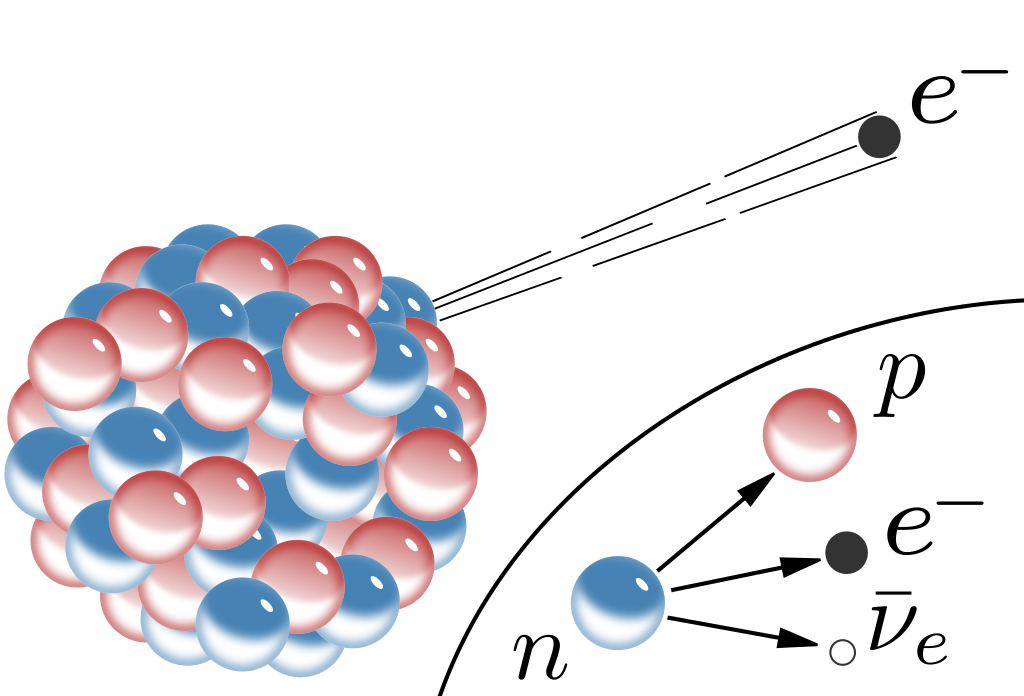
\includegraphics[width=0.9\linewidth,height=0.9\textheight,keepaspectratio]{assets/beta-decay.png}
\caption*{Beta decay and antineutrino production. Source: Beta\_Decay@Wikipedia}
\end{figure}


\end{frame}




\begin{frame}{What are Neutrinos?}

\begin{minipage}[\textheight]{\textwidth}
\begin{columns}[T]

\begin{column}{0.6\textwidth}
\begin{figure}
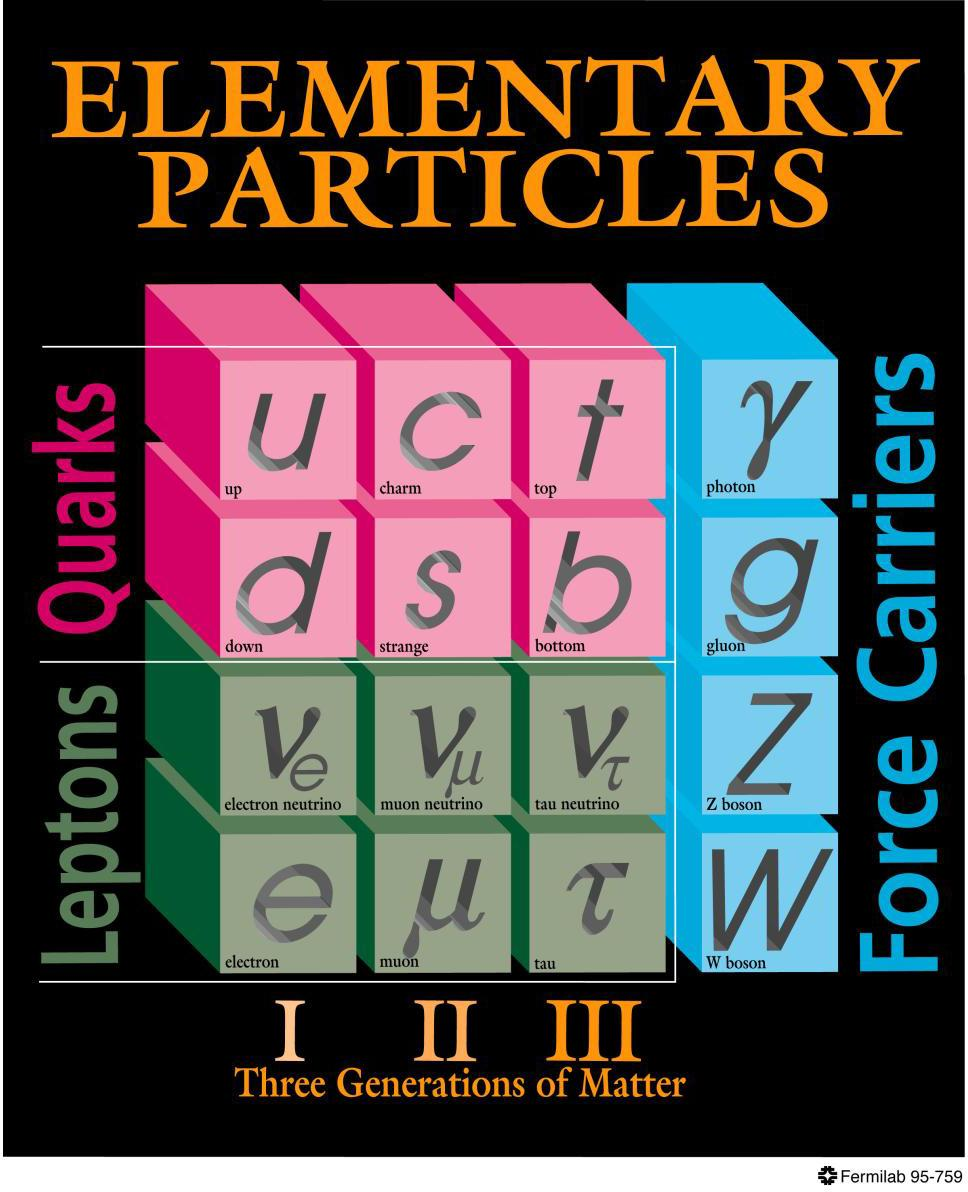
\includegraphics[width=0.9\linewidth,height=0.8\textheight,keepaspectratio]{assets/elementary-particles.jpg}
\caption*{Table of elementary particles. Source: Fermilab} % http://www-d0.fnal.gov/Run2Physics/WWW/results/final/TOP/T06C/T06C.html
\end{figure}
\end{column}

\begin{column}{0.4\textwidth}


    \begin{itemize}
    \item[] Neutrinos are
    \item fermions,
    \item electrically neutral,
    \item light.
    \end{itemize}



\only<1-1>{
\begin{figure}
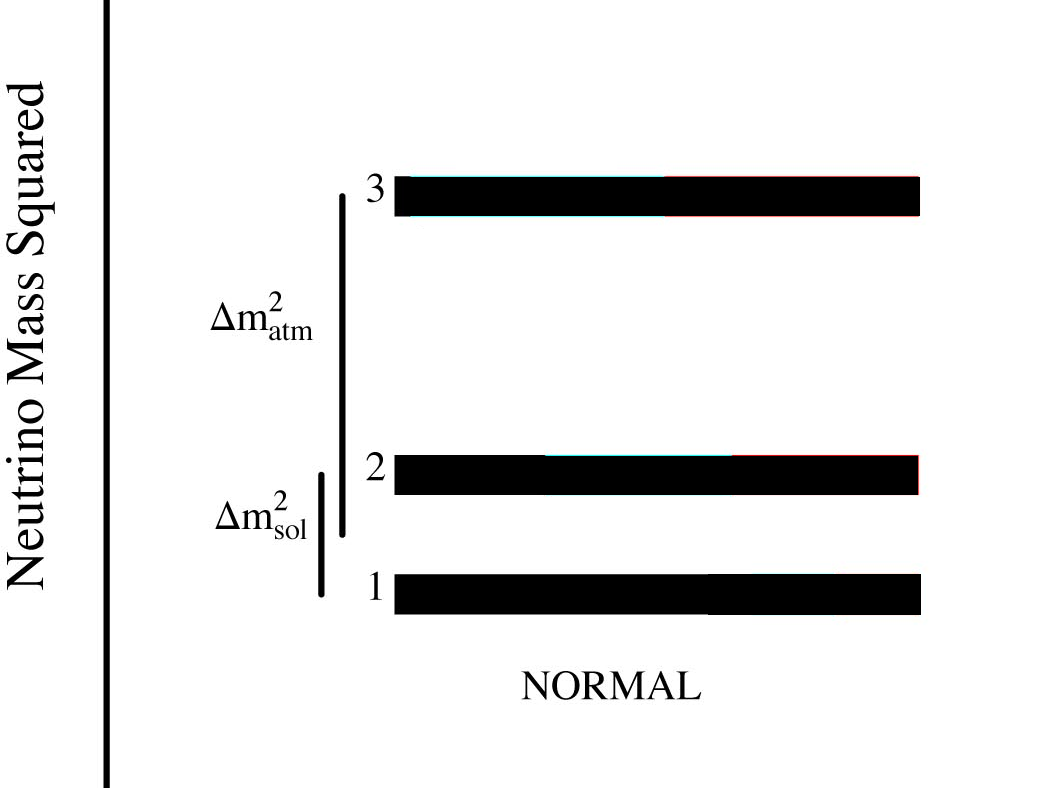
\includegraphics[width=\textwidth]{assets/neutrino-mass-normal-hierarchy-simple.png}
\caption*{Adapted from Olga Mena \& Stephen Parke (2004)}
\end{figure}
}

\only<2-2>{
\begin{figure}
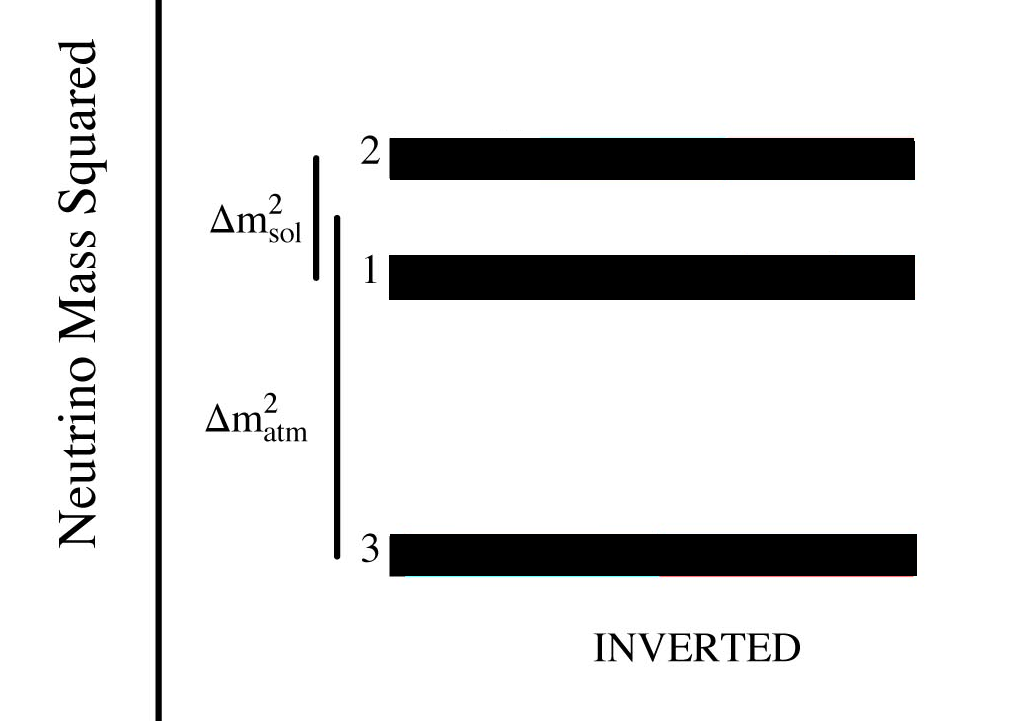
\includegraphics[width=\textwidth]{assets/neutrino-mass-inverted-hierarchy-simple.png}
\caption*{Adapted from Olga Mena \& Stephen Parke (2004)}
\end{figure}
}

\end{column}


\end{columns}
\end{minipage}

\end{frame}



%%%%% Neutrino Oscillations %%%%%%%%%

\subsection{Neutrino Oscillations}





\begin{frame}{What Are Neutrino Oscillations?}




\only<1-1>{

\begin{tcolorbox}
\begin{equation*}
  \equalto{\textbf{\large Neutrino Oscillations} }{ \textbf{\large Neutrino Flavor Conversions } }
\end{equation*}

\end{tcolorbox}


\begin{figure}
    \centering
    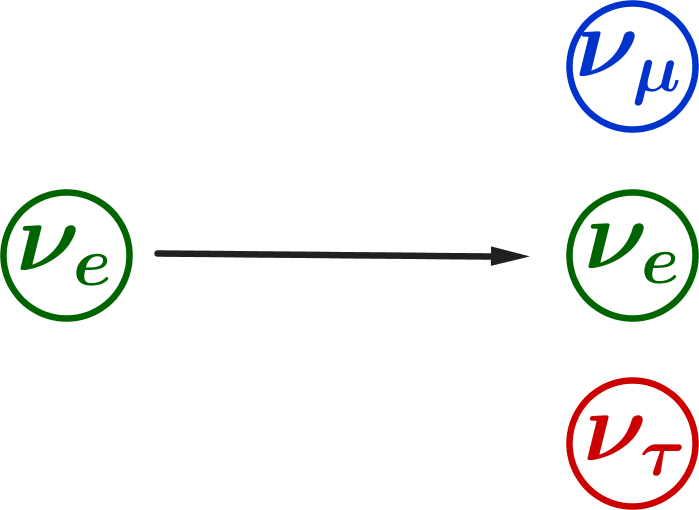
\includegraphics[width=0.6\textwidth]{assets/neutrino-oscillations-illustration}
    \caption*{Neutrino Oscillations}
\end{figure}

}


\only<2-2>{

\begin{figure}
    \centering
    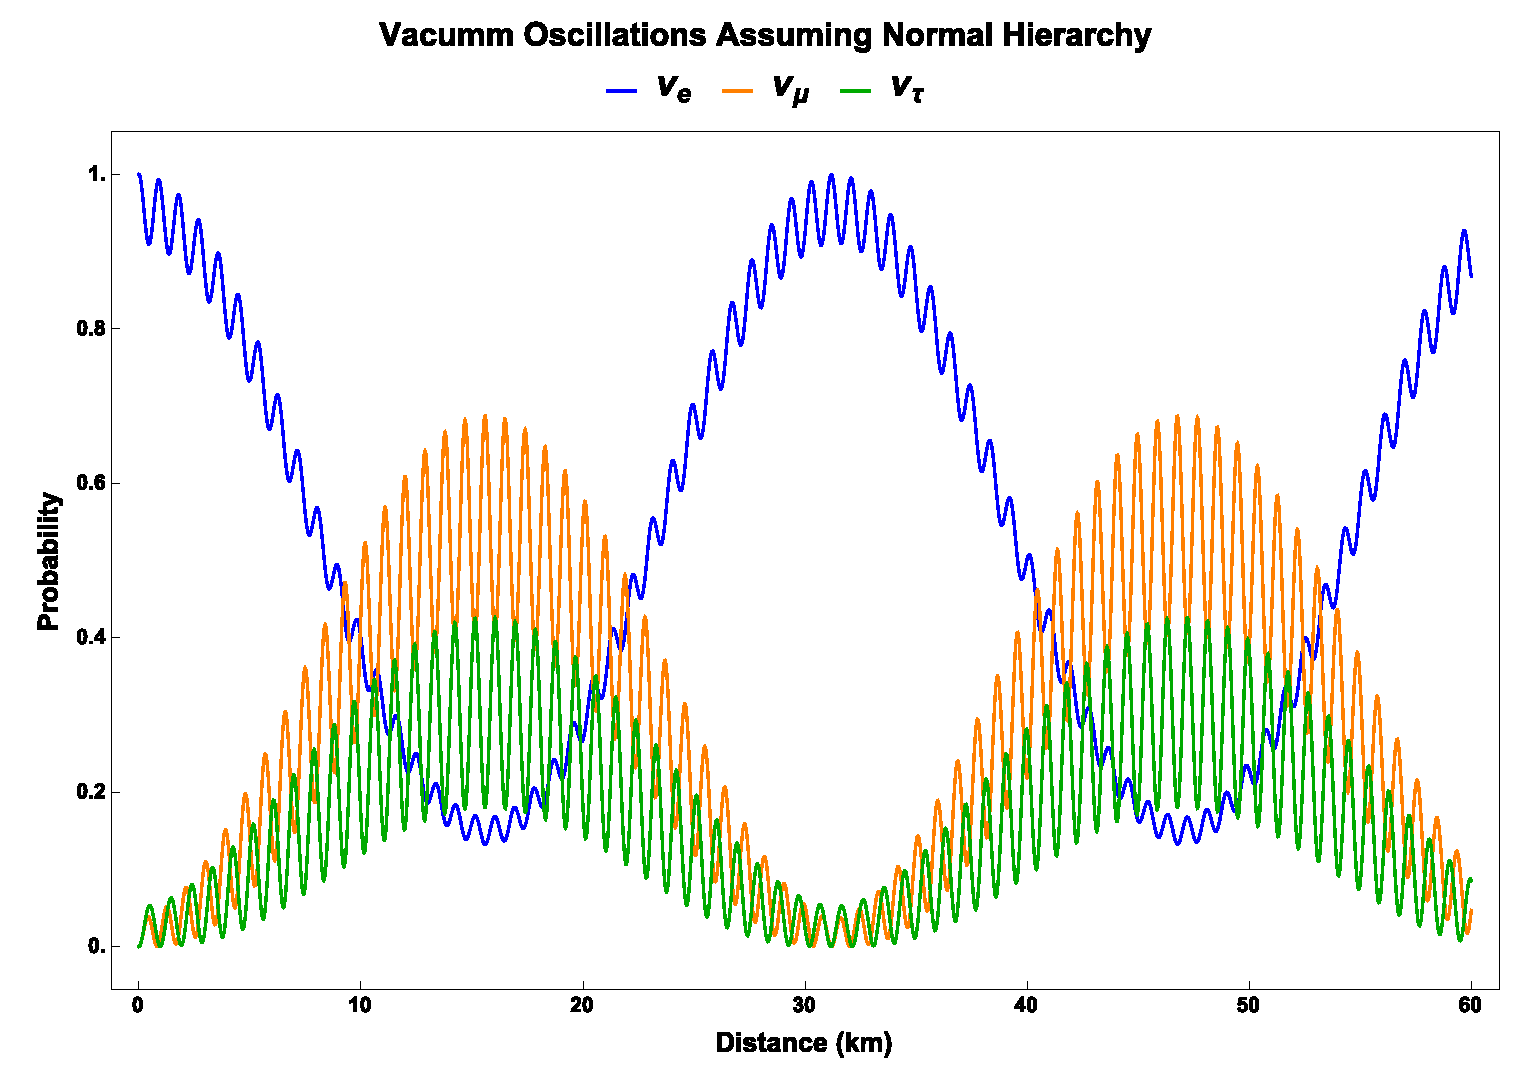
\includegraphics[width=0.9\textwidth]{assets/vacuum-oscillations-3-flavor}
    \caption*{Probabilities of finding neutrinos to be in each flavor.}
    %Neutrino energy: 1MeV}
\end{figure}

}




\end{frame}







%%%%%% Why Neutrinos Oscillate? %%%%%%%%%

\subsection{Why Do Neutrinos Oscillate}

% For every picture that defines or uses external nodes, you'll have to
% apply the 'remember picture' style. To avoid some typing, we'll apply
% the style to all pictures.
\tikzstyle{every picture}+=[remember picture]

% By default all math in TikZ nodes are set in inline mode. Change this to
% displaystyle so that we don't get small fractions.
\everymath{\displaystyle}



\begin{frame}[fragile]{Why Do Neutrinos Oscillate?}
\setbeamercovered{invisible}

\begin{tcolorbox}[title=Equation of Motion]

\begin{equation*}
i\partial_x \begin{pmatrix}
\psi_e\\
\psi_\mu
\end{pmatrix} = \mathbf{H}\begin{pmatrix}
\psi_e\\
\psi_\mu
\end{pmatrix}
\end{equation*}

\end{tcolorbox}

\pause

\begin{tcolorbox}
\begin{equation*}
\mathbf{H} = \frac{\omega_{\mathrm v} }{2}\left( - \cos 2\theta_{\mathrm v } \boldsymbol{\sigma}_3  + \sin 2\theta_{\mathrm{v}} \boldsymbol{\sigma}_1\ \right)
\end{equation*}


\begin{itemize}
    \item Oscillation frequency:
\begin{equation*}
    \omega_{\mathrm v} = \frac{\delta m^2}{2E}=\frac{m_2^2 - m_1^2}{2E}
\end{equation*}
\item Mixing angle $\theta_{\mathrm v}$
\end{itemize}


\end{tcolorbox}






\end{frame}




\begin{frame}{Flavor Isospin}
\setbeamercovered{invisible}







\begin{columns}[T]
\begin{column}{0.5\textwidth}


Hamiltonian: $\mathbf H = - \frac{\vec{\boldsymbol{\sigma}} }{2}\cdot \vec H$


Wave function: $\vec s = \Psi^{\dagger} \frac{\vec{\boldsymbol{\sigma}} }{2} \Psi $


Equation of motion

\begin{equation*}
\dot{\vec s} = \vec s \times \vec H
\end{equation*}


\end{column}%
\begin{column}{0.5\textwidth}


\begin{figure}
    \centering
    \vspace*{-10pt}
    \includegraphics[width=\textwidth]{assets/flavor-isospin-illus}
\end{figure}


\end{column}
\end{columns}

\pause


\begin{columns}[T]
\begin{column}{0.5\textwidth}

Vacuum oscillation Hamiltonian

\begin{align*}
&\frac{\omega_{\mathrm v} }{2}\left( - \cos 2\theta_{\mathrm v } \boldsymbol{\sigma}_3  + \sin 2\theta_{\mathrm{v}} \boldsymbol{\sigma}_1\ \right)\\
\to & \cos 2\theta_{\mathrm v}\begin{pmatrix}
0\\
0\\
\omega_{\mathrm v}
\end{pmatrix} -\sin 2\theta_{\mathrm v}\begin{pmatrix}
\omega_{\mathrm v}\\
0\\
0
\end{pmatrix}
\end{align*}


\end{column}%
\begin{column}{0.5\textwidth}


\begin{figure}
    \centering
    \vspace*{-20pt}
    \includegraphics[width=0.7\textwidth]{assets/flavor-isospin-1}
\end{figure}



\end{column}
\end{columns}




\end{frame}



%%%%%%%%%%%%%%%%%%%%%%%%%%%%%%%%%%%%%%%%%%%%%%%%%%%%%%%%%%%%%%%%%%
%%%%%%%%%%%%%%%%%%%% Matter Effect %%%%%%%%%%%%%%%


\section{Matter Effect}


\subsection{Matter Interactions}


\begin{frame}{Matter Interactions}


% \begin{tcolorbox}[title=PLACEHOLDER]
% SHOULD ADD IN WHY MATTER INTERACTION IS LIKE THIS.
% \end{tcolorbox}


\begin{figure}[ht]
\centering
\begin{minipage}[b]{0.5\linewidth}
\centering
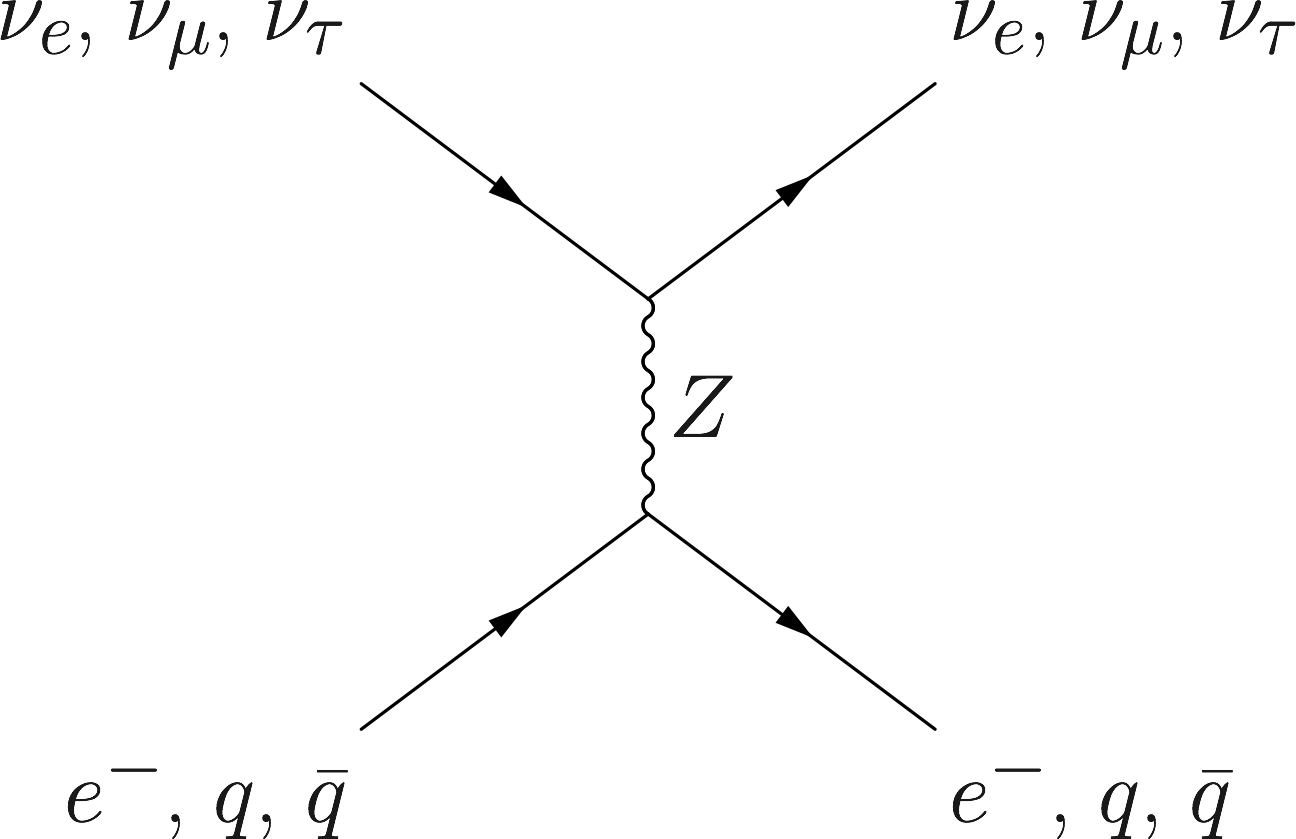
\includegraphics[height=0.42\textheight]{assets/neutral-current.png}
\caption*{Neutral current interaction between\\
$\nu_{\mathrm e}$, $\nu_{\mu}$, $\nu_{\tau}$, 
and $e^{-}$, quarks etc.}
\end{minipage}%
\begin{minipage}[b]{0.5\linewidth}
\centering
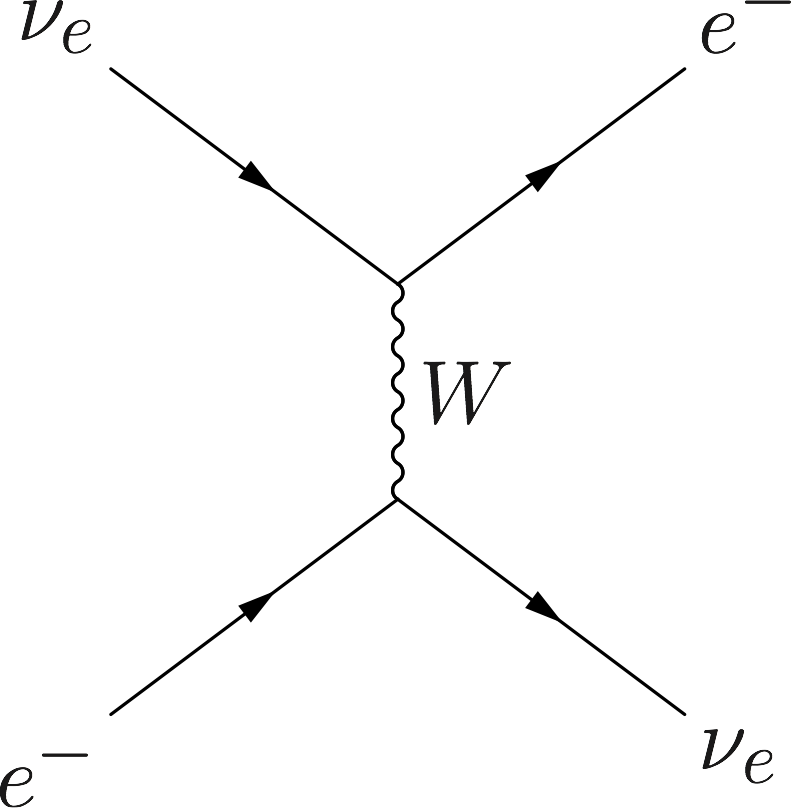
\includegraphics[height=0.42\textheight]{assets/charged-current.png}
\caption*{Charged current interaction between $\nu_{\mathrm e}$ and $e^{-}$}
\end{minipage}
\end{figure}


% \begin{figure}
%     \centering
%     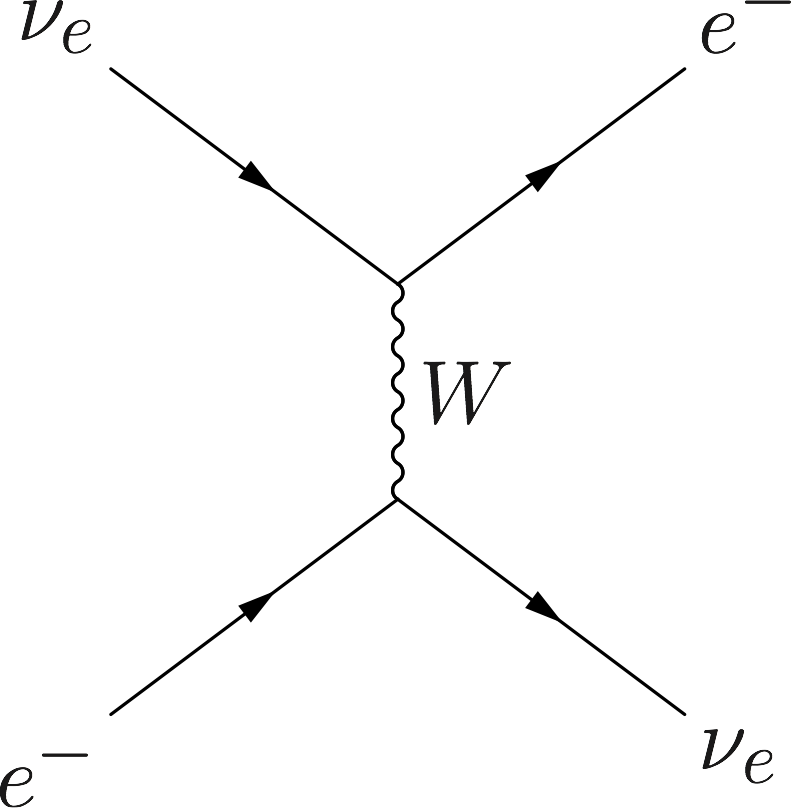
\includegraphics[width=0.5\textwidth]{assets/charged-current.png}
%     \caption*{Interaction between $\nu_{\mathrm e}$ and $e^{-}$}
% \end{figure}


\end{frame}





% For every picture that defines or uses external nodes, you'll have to
% apply the 'remember picture' style. To avoid some typing, we'll apply
% the style to all pictures.
\tikzstyle{every picture}+=[remember picture]


% By default all math in TikZ nodes are set in inline mode. Change this to
% displaystyle so that we don't get small fractions.
\everymath{\displaystyle}



\begin{frame}{Matter Interaction}
\setbeamercovered{invisible}

\tikzstyle{na} = [baseline=-.5ex]




\begin{itemize}
    \item[] Hamiltonian with matter interaction in flavor basis  ($\omega_{\mathrm{v}}=\delta m^2/2E$):
        \tikz[na] \node[coordinate] (n1) {};
\end{itemize}


% \only<1-1>{
% \begin{equation*}
%     \mathbf{H} = 
%     \tikz[baseline]{
%             \node[fill=blue!20,anchor=base] (t1)
%             {$ \frac{\omega_{\mathrm{v}}}{2}\begin{pmatrix} -\cos 2\theta_{\mathrm{v}} & \sin 2 \theta_{\mathrm{v}} \\ \sin 2\theta_{\mathrm{v}} & \cos 2\theta_{\mathrm{v}}  \end{pmatrix} $}
%             } 
%             \tikz[baseline]{
%             \node[fill=red!20, anchor=base] (t2)
%             {$ 
%             \pm \sqrt{2}G_{\mathrm{F}} n_{\mathrm{e}}(x) \begin{pmatrix}
%             1 & 0 \\
%             0 & 0
%             \end{pmatrix}
%             $};
%         }
% \end{equation*}



% }



\only<1->{
\begin{equation*}
    \mathbf{H} = 
    \tikz[baseline]{
            \node[fill=blue!20,anchor=base] (t1)
            {$ \frac{\omega_{\mathrm{v}}}{2}\left( - \cos 2\theta_{\mathrm{v}} \boldsymbol{\sigma_3} + \sin 2\theta_{\mathrm{v}} \boldsymbol{\sigma_1} \right) $}
            } 
            \tikz[baseline]{
            \node[fill=red!20, anchor=base] (t2)
            {$ 
            +\frac{\lambda(x)}{2} \boldsymbol{\sigma_3}
            $};
        }
\end{equation*}

}


\begin{itemize}
    \item Vacuum Hamiltonian
        \tikz[na]\node [coordinate] (n2) {};
    \item Matter interaction
        \tikz[na]\node [coordinate] (n3) {};
    \item<2-> $\lambda(x) = \sqrt{2}G_{\mathrm{F}} n_{\mathrm{e}}(x)$ 
\end{itemize}





% Now it's time to draw some edges between the global nodes. Note that we
% have to apply the 'overlay' style.
\begin{tikzpicture}[overlay]
        \path[->]<1-> (n2) edge [bend right] (t1);
        \path[->]<1-> (n3) edge [bend right=20] (t2);
\end{tikzpicture}




\end{frame}

% \begin{frame}{Matter Interaction}


% \begin{tcolorbox}[title=Hamiltonian with Matter Potential]

% \begin{equation*}
%     \mathbf{H} = 
% \end{equation*}

% \end{tcolorbox}



% \end{frame}





%%%%%%%%%%%%%%%%%
\subsection{MSW Effect}

\begin{frame}{MSW Effect}

\begin{align*}
    \mathbf H =& \colorbox{blue!20}{$ \frac{\omega_{\mathrm{v}}}{2}\left( - \cos 2\theta_{\mathrm{v}} \boldsymbol{\sigma_3} + \sin 2\theta_{\mathrm{v}} \boldsymbol{\sigma_1} \right) $}   \colorbox{red!20}{$ + \frac{\lambda(x)}{2} \boldsymbol{\sigma_3} $} \\
    \to &  \colorbox{blue!20}{$ \omega_{\mathrm v}\begin{pmatrix}
    - \sin 2\theta_{\mathrm v} \\
    0 \\
    \cos 2\theta_{\mathrm v}
    \end{pmatrix} $}  \colorbox{red!20}{$ + \begin{pmatrix}
    0\\
    0\\
    - \lambda(x)
    \end{pmatrix} $} \\
    \to &  \colorbox{blue!20}{$ \vec H_{\mathrm v} $}  \colorbox{red!20}{$ + \vec H_{\mathrm m}(x) $}
\end{align*}






\end{frame}



\begin{frame}{MSW Effect}


\only<1>{

\begin{columns}[T]
\begin{column}{0.5\textwidth}

\begin{figure}
    \centering
    \includegraphics[width=0.4\textwidth]{assets/matter-effect-large-density}
\end{figure}


\end{column}%
\begin{column}{0.5\textwidth}


\begin{figure}
    \centering
    \includegraphics[width=0.6\textwidth]{assets/matter-effect-notsolarge-density}
\end{figure}



\end{column}
\end{columns}

}

\only<2> {


\begin{columns}[T]
\begin{column}{0.5\textwidth}

\begin{figure}
    \centering
    \includegraphics[width=0.9\textwidth]{assets/matter-effect-critical-density}
\end{figure}


\end{column}%
\begin{column}{0.5\textwidth}


\begin{figure}
    \centering
    \includegraphics[width=0.9\textwidth]{assets/matter-effect-small-density}
\end{figure}



\end{column}
\end{columns}


}




\end{frame}








%%%%%%%%%%%%%%%%%%%%%%%%%%%%%%%%%%%%%%%%%%%%%%%%%%%%%%%%%%%%%%%%%%
%%%%%%%%%%%%%%%%%%%% Parametric Effect %%%%%%%%%%%%%%%


% \begin{frame}{Parametric Effect}

% \begin{tcolorbox}[title=Parametric Effect]

% Parametric Effect, Parametric Resonance?

% \end{tcolorbox}

% \end{frame}


%%%%%%%%%%%%%%%%%%%%%%%%%%%%%%%%%%%%%%%%%%%%%%%%%%%%%%%%%%%%%%%%%%
%%%%%%%%%%%%%%%%%%%% Stimulated Effect/Multi-frequency stimulation %%%%%%%%%%%%%%%

\subsection{Stimulated Neutrino Oscillations}

% \begin{frame}{Length Scales}

% \begin{tcolorbox}[title=Characteristic Scales]
% \begin{itemize}
%     \item Vacuum problem:
%     \begin{equation*}
%         l_{\mathrm v} \sim \frac{1}{\omega_{\mathrm v}}
%     \end{equation*}
    
%     \item Constant matter profile $\lambda_0$:
%     \begin{equation*}
%         l_{\mathrm v}, \quad l_{\mathrm m} \sim \frac{1}{\omega_{\mathrm m}} 
%     \end{equation*}
    
%     \item Varying matter profile $\lambda(x) = \lambda_0 + A \sin (k x)$,
    
%     \begin{equation*}
%         l_{\mathrm v}, \quad l_{\mathrm m}, \quad l_{k} \sim \frac{1}{k}
%     \end{equation*}
% \end{itemize}

% \end{tcolorbox}

% % \only<2-2>{
% % \begin{textblock*}{64mm}(64mm,0.01\textheight)

% % \tiny
% % $$\omega_{\mathrm m} = \omega_{\mathrm v}\sqrt{ \left(\frac{\lambda}{\omega_{\mathrm v}} - \cos 2\theta_{\mathrm v} \right)^2 + \sin^2 2\theta_{\mathrm v}  }$$
% % \normalsize

% % \end{textblock*}
% % }


% \only<1>{
% \begin{tcolorbox}[title=MSW Resonance]


% \begin{equation*}
%     l_{\mathrm v} \sim l_{\mathrm m} \sin 2\theta_{\mathrm v}
% \end{equation*}

% \end{tcolorbox}
% }

% \only<2-2>{

% \begin{tcolorbox}[title=Other Resonance?]
% \centering
% $l_{\mathrm m}$, and $l_{k}$?

% \end{tcolorbox}

% }



% \end{frame}



\begin{frame}{More Complicated Matter Effect}

\begin{tcolorbox}[title=Why Do We Care]

Astrophysical environments: supernovae, accretion disks etc

\end{tcolorbox}

\begin{figure}
    \centering
    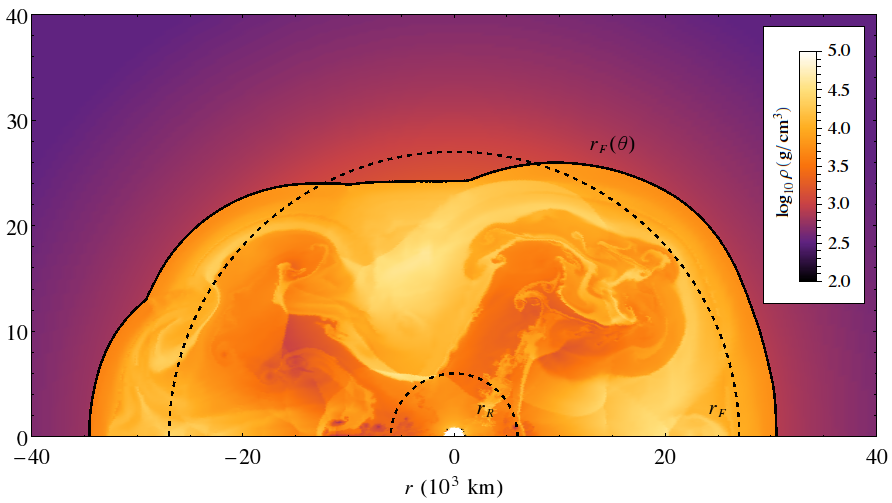
\includegraphics[height=0.5\textheight]{assets/supernova-shock-turbulence.png}
    \caption*{Supernova shock and turbulence. E. Borriello, et al  (2014)}
    %https://inspirehep.net/record/1262293?ln=en
    % arXiv: 1310.7488
\end{figure}

\vspace{-1em}
\begin{equation*}
\Delta n_e (r) = \sum_n c_n \sin( k_n r + \phi_n )
\end{equation*}
    

\end{frame}






    



\begin{frame}{Stimulated Neutrino Oscillations}


\only<1-1>{

\begin{textblock*}{10pt}(280pt,1pt)
\small
\begin{equation*}
\lambda(x) =\sqrt{2}G_{\mathrm F}n_e    
\end{equation*}

\end{textblock*}




\begin{tcolorbox}[title=Matter Profile]
\begin{align*}
    &n_e(x) = n_0 + \delta n \sin(k x + \phi) \\
    \Rightarrow & \lambda(x) = \lambda_0 + \delta \lambda \sin(k x + \phi)
\end{align*}
\end{tcolorbox}

}

\only<2-2>{

% \begin{tcolorbox}
% Kneller, J. P., McLaughlin, G. C., \& Patton, K. M. (2013). J. Phys. G: Nucl. Part. Phys. {\bf{40}} (2013) 055002.
% \end{tcolorbox}

\begin{tcolorbox}
P. Krastev and A. Smirnov (1989); J. Kneller et al (2013);\\ K. Patton et al (2014);
\end{tcolorbox}


\begin{figure}
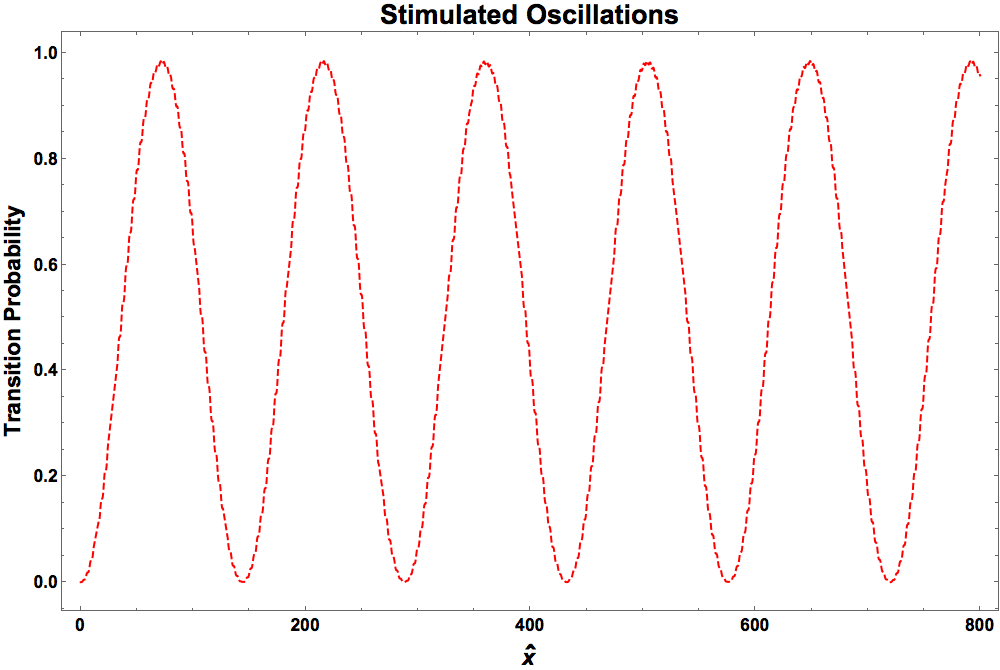
\includegraphics[width=0.8\textwidth]{assets/stimulated-oscillation-phenomenon.png}
%stimulated-neutrino-oscillations-kneller.png}
\caption*{Stimulated oscillations. $\lambda(x) = \lambda_0 +  A \sin (k x)$  with $\hat x = \omega_{\mathrm m} x $, $A=0.1\omega_{\mathrm m}$, $k=0.995\omega_{\mathrm m}$, $\theta_{\mathrm{m}}=\pi/6$}
\end{figure}


}



% %%% A text block that should be displayed later
% \only<3->{
% \begin{textblock*}{64mm}(32mm,0.4\textheight)

% \begin{tcolorbox}
% \centering
% %\rotatebox{0}{
% ${\color{red}\delta\lambda(x)}$ is the problem here.
% \begin{itemize}
%     \item Varying background eigenenergy
%     \item $\cdots$
% \end{itemize}
% %}
% \vspace{1em}
% \end{tcolorbox}

% \end{textblock*}
% }


\end{frame}









\section{Stimulated Neutrino Flavor Transitions}


\subsection{Rabi Oscillations}






%%%%%%%%%%%%%%%%%%%%%%%%%%%%%%%%
% Intuitive Demonstration BEGIN
%%%%%%%%%%%%%%%%%%%%%%%%%%%%%%%%




\subsection{Rabi Oscillations}

\begin{frame}{Rabi Oscillations}
\setbeamercovered{invisible}



 
\only<1,4>{
  
\begin{columns}[T]
\begin{column}{0.4\textwidth}
\begin{tcolorbox}[title=Rabi Oscillation]

Hamiltonian

\begin{equation*}
    -\frac{\omega_{\mathrm m}}{2} \sigma_3 - \frac{\alpha}{2} \begin{pmatrix}
    0 & e^{ikt}\\
    e^{-ikt} & 0
    \end{pmatrix}
\end{equation*}
\end{tcolorbox}

\end{column}%
\begin{column}{0.6\textwidth}
\begin{figure}
    \centering
    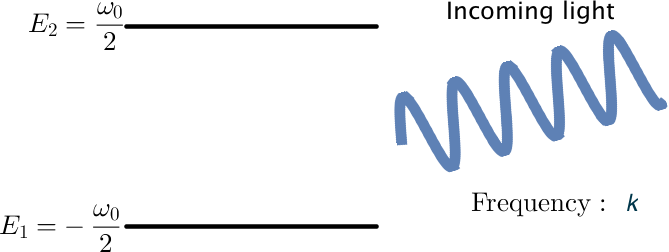
\includegraphics[width=\textwidth]{assets/rabi-diagram.png}
\end{figure}


\end{column}
\end{columns}



}


\only<2>{



\begin{columns}[T]
\begin{column}{0.5\textwidth}

\begin{equation*}
    \vec H_3 = \omega_{\mathrm m}\begin{pmatrix}
    0 \\
    0\\
    1
    \end{pmatrix}, \vec H_+ = \alpha  \begin{pmatrix}
    \cos( kt) \\
    -\sin(kt)\\
    0
    \end{pmatrix}
\end{equation*}


\end{column}%
\begin{column}{0.5\textwidth}

\begin{equation*}
    \vec H'_3 = (\omega_{\mathrm m} - k)\begin{pmatrix}
    0 \\
    0\\
    1
    \end{pmatrix}, \vec H'_+ = \alpha  \begin{pmatrix}
    1 \\
    0\\
    0
    \end{pmatrix}
\end{equation*}





\end{column}
\end{columns}


}

\only<2>{

\begin{columns}[T]
\begin{column}{0.5\textwidth}




\begin{figure}
    \centering
    \includegraphics[width=0.8\textwidth]{assets/rabi-isospin-static-frame}
\end{figure}

\end{column}%
\begin{column}{0.5\textwidth}



\begin{figure}
    \centering
    \includegraphics[width=0.8\textwidth]{assets/rabi-isospin-rotating-frame}
\end{figure}



\end{column}
\end{columns}

}

\only<3>{


\begin{equation*}
    \vec H'_3 = (\omega_{\mathrm m} - k)\begin{pmatrix}
    0 \\
    0\\
    1
    \end{pmatrix} = 0
\end{equation*}


\begin{figure}
    \centering
    \includegraphics[width=0.5\textwidth]{assets/rabi-isospin-rotating-frame-resonance}
\end{figure}


}



\only<4>{



Rabi formula

\begin{equation*}
    P_{1\to 2} = \frac{1}{1 + D^2} \sin^2 \left( \frac{\Omega_{\mathrm R}}{2} t \right).
\end{equation*}

Relative detuning

\begin{equation*}
    D = \left\vert\frac{\omega_{\mathrm m} - k}{\alpha} \right\vert.
\end{equation*}

Rabi frequency

\begin{equation*}
\Omega_{\mathrm R} = \sqrt{\colorbox{red!20}{$\alpha$}^2+(\colorbox{blue!20}{$\omega_{\mathrm m} - k$})^2}    
\end{equation*}



}


\end{frame}




\begin{frame}{Rabi Oscillations}


\begin{figure}
    \centering
    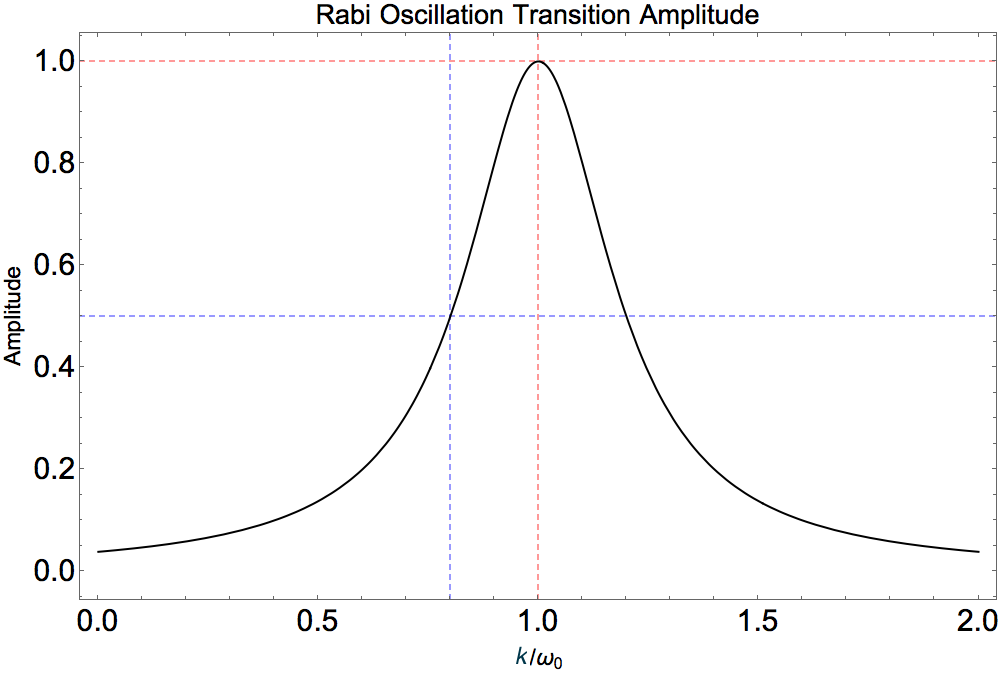
\includegraphics[width=0.9\textwidth]{assets/rabi-resonance.png}
    \caption*{Amplitude of Rabi oscillations for different driving field frequency $k$}
\end{figure}



\end{frame}





\subsection{Single Frequency Matter Profile and Rabi Oscillations}


\begin{frame}{Hamiltonian in Matter Basis}


% Matter profile
\begin{tcolorbox}[title=Matter Profile]
\begin{equation*}
    \lambda(x)  = \lambda_0 \only<2>{ + {\color{red}A\sin(k x)} }
\end{equation*}
\end{tcolorbox}


% Basis


\begin{tcolorbox}[title=Basis]

Background matter basis (eigen energy basis): Hamiltonian is diagonalized with only background matter profile $\lambda_0$,

\begin{equation*}
    \mathrm{H}_{\mathrm{background}} = -\frac{\omega_{\mathrm{m}}}{2} \boldsymbol{\sigma_3}.
\end{equation*}

\end{tcolorbox}


% Hamiltonian of with perturbation in matter profile, in background matter basis
\begin{tcolorbox}[title=Hamiltonian]

\begin{equation*}
    \mathbf H = \frac{1}{2}\left( - \omega_{\mathrm{m}} 
    \only<2>{
    + {\color{red}A\sin(kx)} \cos 2\theta_{\mathrm{m}} 
    } 
    \right) \boldsymbol{\sigma_3} 
    \only<2>{
    - \frac{{\color{red}A\sin(kx) } }{2} \sin \theta_{\mathrm{m}} \boldsymbol{\sigma_1}
    }
\end{equation*}


\end{tcolorbox}






\end{frame}






\begin{frame}{Hamiltonian in Matter Basis}

\begin{align*}
    \mathbf {H} =& \frac{1}{2}\left( - \omega_{\mathrm{m}} \colorbox{gray!20}{$+  \cos 2\theta_{\mathrm{m}}{\color{red}A\sin(kx)} $} \right) \sigma_3 - \frac{  \sin 2\theta_{\mathrm{m} }  }{2}{\color{red}A \sin(kx)}  \sigma_1 \\
    \to &  \omega_{\mathrm m}\begin{pmatrix}
    0\\
    0\\
    1
    \end{pmatrix} + \alpha \begin{pmatrix}
    \sin (kx)\\
    \cos(k x)\\
    0
    \end{pmatrix}  \colorbox{gray!20}{$+ \alpha \begin{pmatrix}
    \sin (kx)\\
    - \cos(k x)\\
    0
    \end{pmatrix} $}
\end{align*}

where

\begin{equation*}
    \alpha = \frac{\sin2\theta_{\mathrm m}}{2}A
\end{equation*}






\end{frame}



\begin{frame}{Rabi Formula Works}


\begin{textblock*}{10pt}(230pt,-1pt)
{\tiny
\begin{equation*}
\vec H \sim  \omega_{\mathrm m}\begin{pmatrix}
    0\\
    0\\
    1
    \end{pmatrix} + \alpha \begin{pmatrix}
    \sin (kx)\\
    \cos(k x)\\
    0
    \end{pmatrix} 
\end{equation*}
}
\end{textblock*}


\begin{figure}
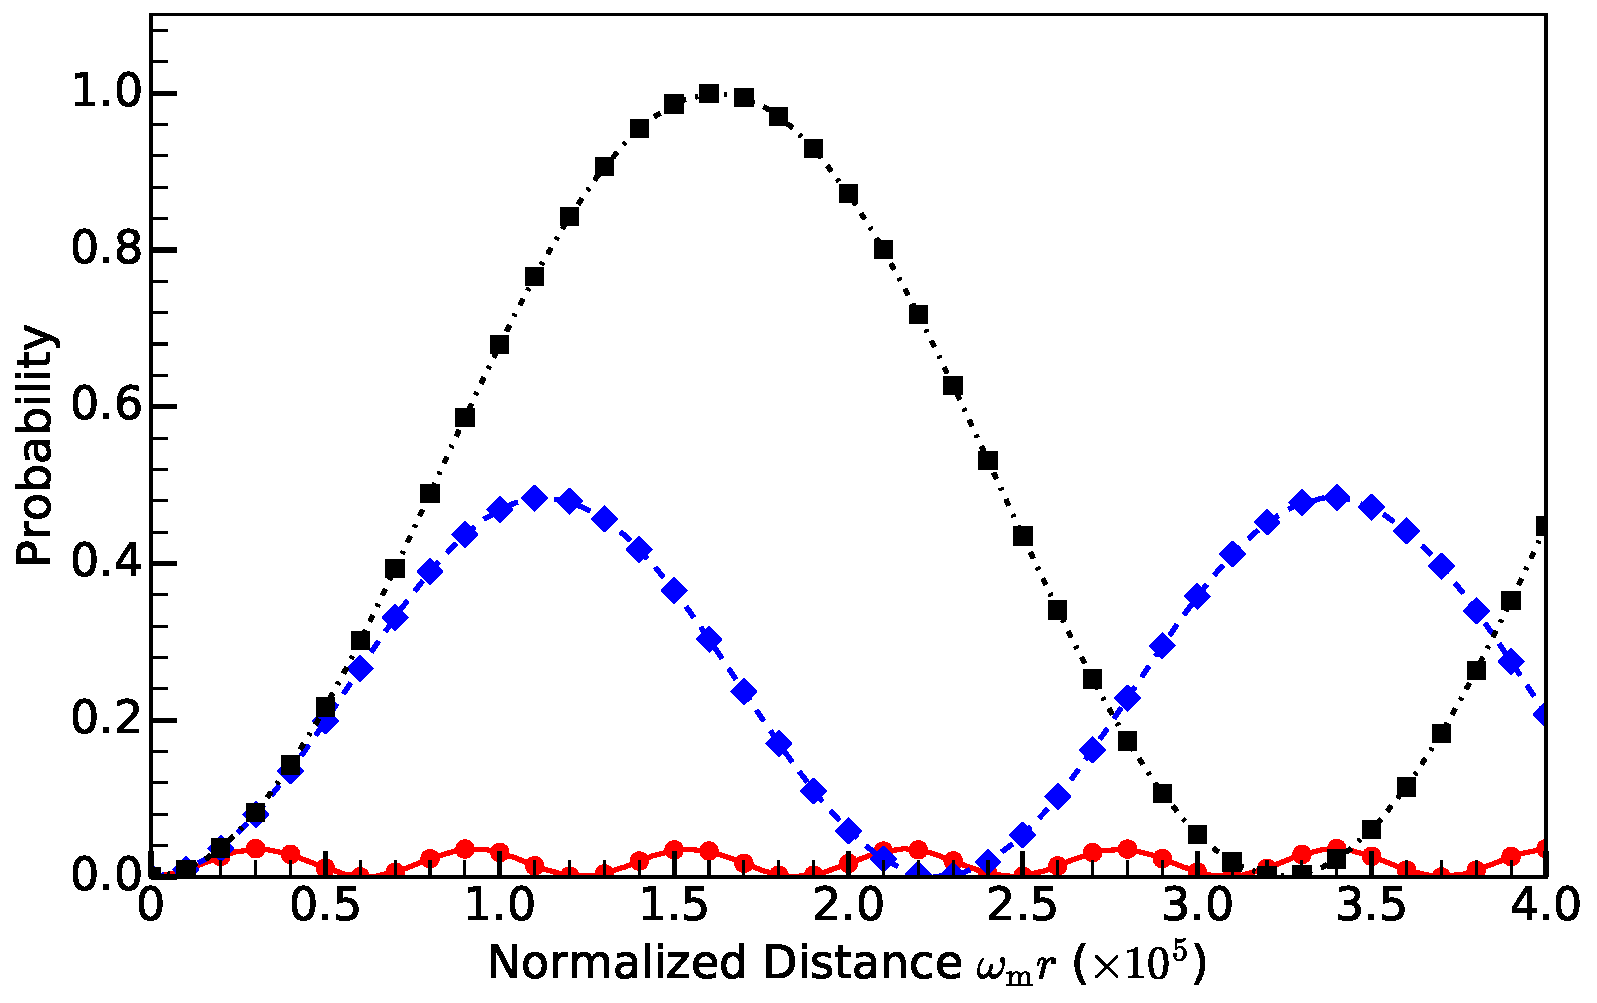
\includegraphics[width=0.9\textwidth]{assets/rabiOscillationsNeutrinoCoincidence-single-frequency}
%stimulated-neutrino-oscillations-kneller.png}
\caption*{
Lines: Rabi formula\\
Dots, diamonds, triangles, and squares are for $k=\omega_{\mathrm m}$, $k=(1-2\times 10^{-5})\omega_{\mathrm m}$, and $k=(1-10^{-4})\omega_{\mathrm m}$ respectively.
}
\end{figure}


\end{frame}


\subsection{Interferences of Rabi Oscillations}


\begin{frame}{Interferences of Rabi Oscillations}


\begin{textblock*}{10pt}(280pt,-1pt)
{\tiny
\begin{equation*}
\alpha = \frac{\sin2\theta_{\mathrm m}}{2}A
\end{equation*}
}
\end{textblock*}



\begin{equation*}
    \vec {H} 
    =  \omega_{\mathrm m}\begin{pmatrix}
    0\\
    0\\
    1
    \end{pmatrix} + \alpha \begin{pmatrix}
    \sin (kx)\\
    \cos(k x)\\
    0
    \end{pmatrix}  \colorbox{gray!20}{$+ \alpha \begin{pmatrix}
    \sin (kx)\\
    - \cos(k x)\\
    0
    \end{pmatrix} $}
\end{equation*}



    



\begin{tcolorbox}
Dropping off-resonance frequency: Requirement?
\end{tcolorbox}


\end{frame}





\begin{frame}{Interferences of Rabi Oscillations}

\only<1>{
\begin{equation*}
    \vec H = \begin{pmatrix}
    0\\
    0\\
    \omega_m
    \end{pmatrix} + \alpha_1\begin{pmatrix}
     \cos(k_1x)\\
    -\sin(k_1x)\\
    0
    \end{pmatrix} + \colorbox{blue!20}{$\alpha_2\begin{pmatrix}
    \cos(k_2x)\\
    -\sin(k_2x)\\
    0
    \end{pmatrix}$}
\end{equation*}

Corotating frame of the second frequency,



\begin{equation*}
    \vec H = \begin{pmatrix}
    0\\
    0\\
    \omega_m - k_2
    \end{pmatrix} + \alpha_1\begin{pmatrix}
     \cos(k_1-k_2x)\\
    -\sin(k_1-K_2x)\\
    0
    \end{pmatrix} + \colorbox{blue!20}{$\alpha_2\begin{pmatrix}
    1\\
    0\\
    0
    \end{pmatrix}$}
\end{equation*}

}

\only<1>{
Energy gap in this frame becomes the length of the vector

\begin{equation*}
    \begin{pmatrix}
    0\\
    0\\
    \omega_m - k_2
    \end{pmatrix} + \colorbox{blue!20}{$\alpha_2\begin{pmatrix}
    1\\
    0\\
    0
    \end{pmatrix}$}
\end{equation*}
}

\only<2->{
Energy gap in this frame becomes the length of the vector
\begin{equation*}
\sqrt{(\omega_{\mathrm m} - k_2)^2 + \alpha_2^2 } \to \omega_{\mathrm m} - k_2 + \frac{1}{2}\frac{\alpha_2^2}{\omega_{\mathrm m}-k_2}
\end{equation*}

Relative detuning

\begin{equation*}
D' =  \left\vert \frac{\omega_{\mathrm m} - k_1 }{\alpha_1} + \frac{\alpha_2^2}{2\alpha_1(\omega_{\mathrm m}-k_2)} \right\vert
\end{equation*}

}

\end{frame}




\begin{frame}{Interferences of Rabi Oscillations}



\begin{textblock*}{10pt}(220pt,16pt)
\small
\begin{equation*}
D' =  \left\vert \frac{\omega_{\mathrm m} - k_1 }{\alpha_1} + \frac{\alpha_2^2}{2\alpha_1(\omega_{\mathrm m}-k_2)} \right\vert
\end{equation*}
\end{textblock*}


\vspace{2em}

Two driving frequencies $k_1$, and $k_2$, with amplitude $\alpha_1$, and $\alpha_2$

Destruction effect: $k_1 = \omega_{\mathrm m}$, $\lvert \alpha_2\rvert \gg \sqrt{ 2\omega_{\mathrm m} \lvert \alpha_1 (k_2 - \omega_{\mathrm m}) \rvert }\equiv \alpha_{2,\mathrm C}$




% \begin{figure}
%     \centering
%     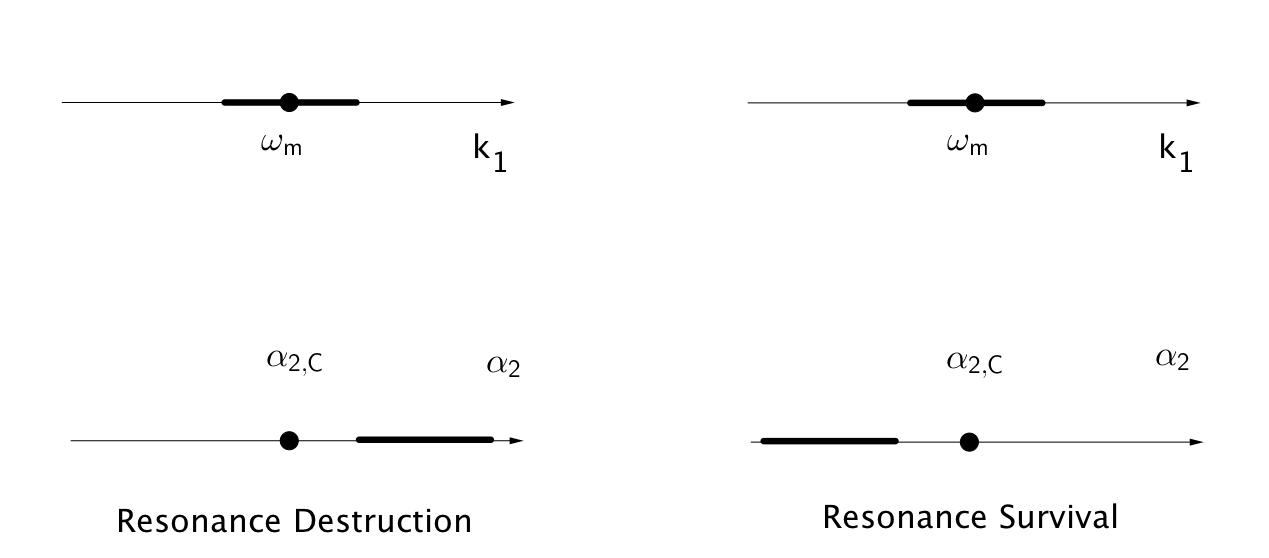
\includegraphics[width=\textwidth,trim={0 0.1cm 0 0.5cm},clip]{assets/rabi-osc-interferenes}
% \end{figure}



\end{frame}


\begin{frame}{Interferences of Rabi Oscillations}


\begin{figure}
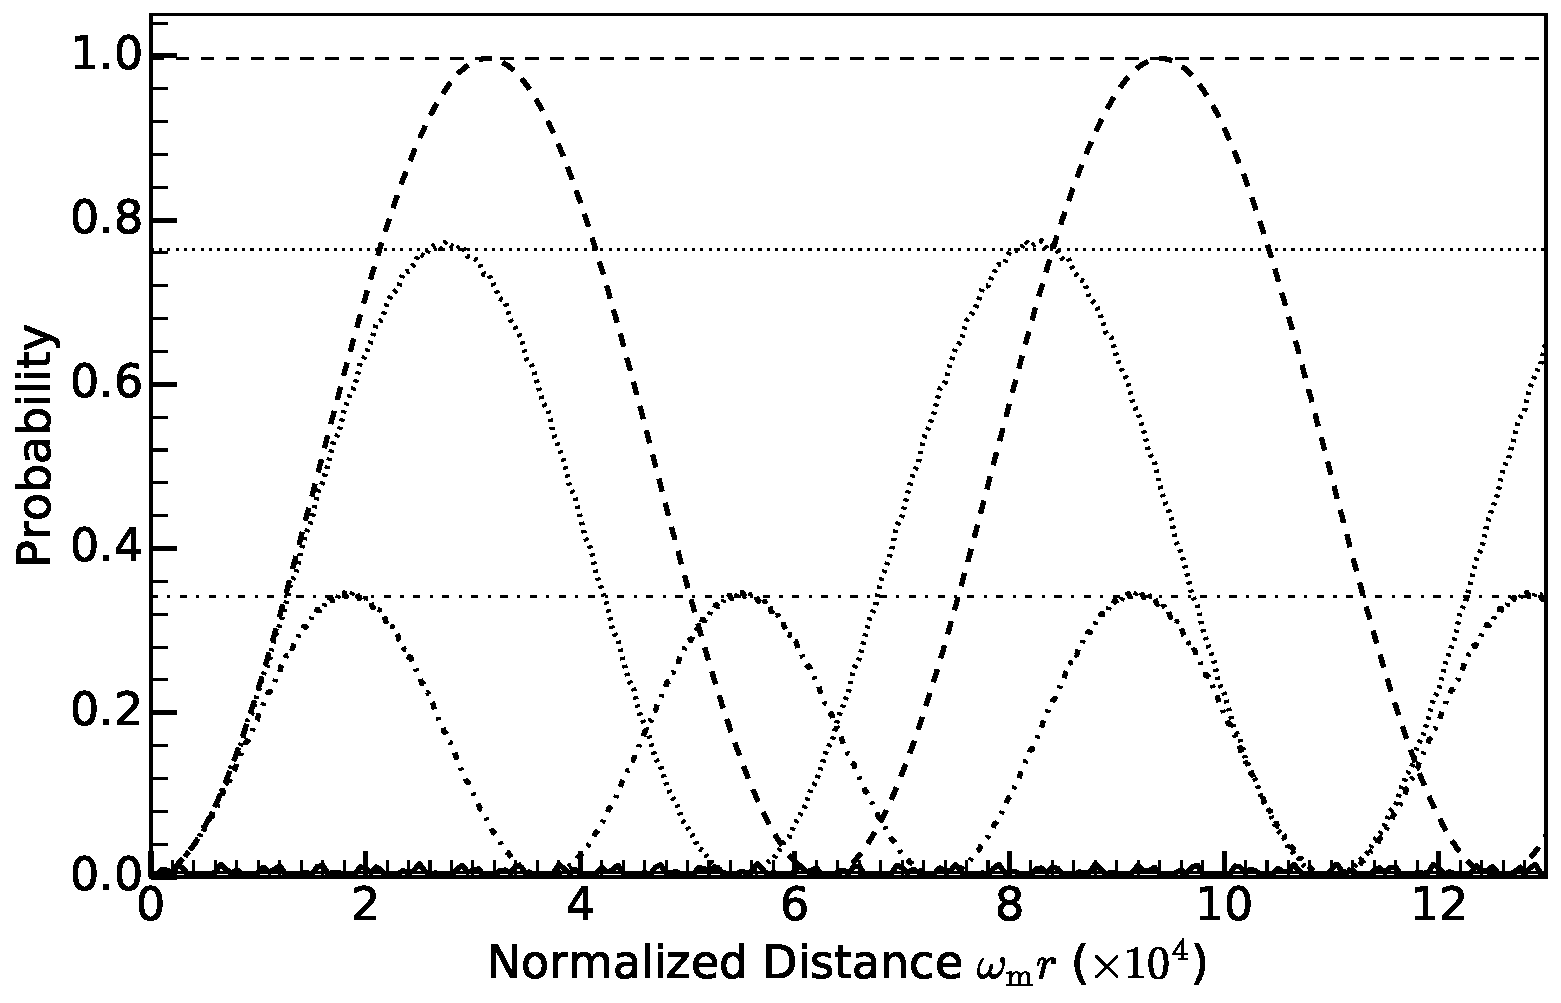
\includegraphics[width=0.9\textwidth]{assets/interference-reduction}
\caption*{Grid lines: amplitude predicted using $1/(1+D'^2)$ 
}
\end{figure}

% Dashed line, dotted line, dash-dotted line, and solid line are for $A_2=10^{-2}\omega_{\mathrm{m}}$, $k_2=10\omega_{\mathrm m}$, $A_2=10^{-2}\omega_{\mathrm{m}}$, $k_2=10^{-1}\omega_{\mathrm m}$, $A_2=5.0\times 10^{-2}\omega_{\mathrm{m}}$, $k_2=10\omega_{\mathrm m}$, and $A_2=5\times 10^{-2}\omega_{\mathrm{m}}$, $k_2=10^{-1}\omega_{\mathrm m}$

{\tiny
\begin{center}
    \begin{tabular}{c|c|c|c}
    \multicolumn{4}{c}{ $\alpha_2$, $k_1$ values} \\
    \hline
       Dashed  &  dotted & dash-dotted & solid \\
       $10^{-2}\omega_{\mathrm{m}}$, $10\omega_{\mathrm m}$  &  $10^{-2}\omega_{\mathrm{m}}$, $10^{-1}\omega_{\mathrm m}$  & $5.0\times 10^{-2}\omega_{\mathrm{m}}$, $10\omega_{\mathrm m}$  & $5\times 10^{-2}\omega_{\mathrm{m}}$, $10^{-1}\omega_{\mathrm m}$
    \end{tabular}
\end{center}
}

\end{frame}



\begin{frame}{Rabi Formula Works}


\begin{textblock*}{10pt}(230pt,-1pt)
{\tiny
\begin{equation*}
\vec H \sim  \omega_{\mathrm m}\begin{pmatrix}
    0\\
    0\\
    1
    \end{pmatrix} + \alpha \begin{pmatrix}
    \sin (kx)\\
    \cos(k x)\\
    0
    \end{pmatrix} 
\end{equation*}
}
\end{textblock*}


\begin{figure}
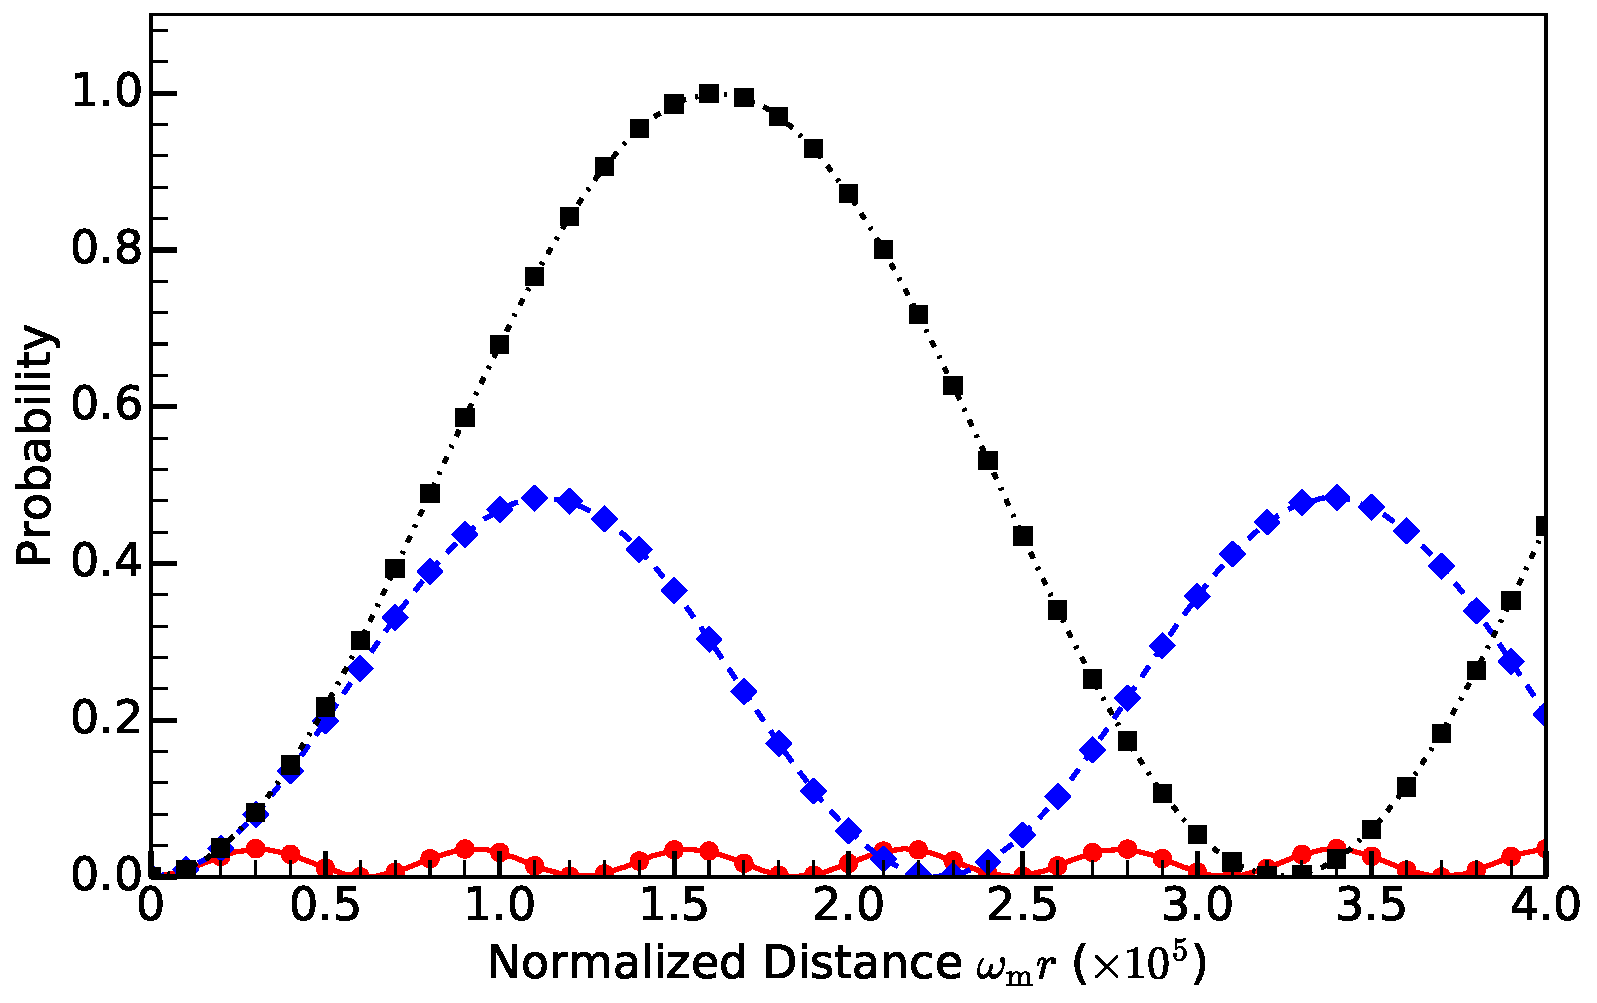
\includegraphics[width=0.9\textwidth]{assets/rabiOscillationsNeutrinoCoincidence-single-frequency}
%stimulated-neutrino-oscillations-kneller.png}
\caption*{
Lines: Rabi formula\\
Dots, diamonds, triangles, and squares are for $k=\omega_{\mathrm m}$, $k=(1-2\times 10^{-5})\omega_{\mathrm m}$, and $k=(1-10^{-4})\omega_{\mathrm m}$ respectively.
}
\end{figure}

\tiny
\centering
$\alpha_{2,\mathrm C} = 2 \alpha = 2 \times \frac{A\sin 2\theta_{\mathrm m}}{2}$


\end{frame}



\section{Jacobi-Anger Expansion}



\begin{frame}{Interferences of Rabi Oscillations}

We have been making approximations.


\begin{align*}
    \mathbf {H} =& \frac{1}{2}\left( - \omega_{\mathrm{m}} \colorbox{gray!20}{$+  \cos 2\theta_{\mathrm{m}}A\cos(kx) $} \right) \sigma_3 - \frac{  \sin 2\theta_{\mathrm{m} }  }{2}A \cos(kx)  \sigma_1\\
    \to& -\frac{\omega_m}{2} \sigma_3 - \frac{A\sin 2\theta_{\mathrm m}}{2} \cos(kx)\sigma_1 
\end{align*}

We need a better basis.



\end{frame}



\subsection{Basis and Formalism}



\begin{frame}{Rabi Basis}



\begin{tcolorbox}[title=Hamiltonian in Background Matter Basis]
    \begin{equation*}
    \mathbf {H} = \frac{1}{2}\left( - \omega_{\mathrm{m}} + {\color{red}\delta \lambda(x)} \cos 2\theta_{\mathrm{m}} \right) \boldsymbol{\sigma_3} - \frac{  {\color{red}\delta \lambda(x)}  }{2} \sin \theta_{\mathrm{m}} \boldsymbol{\sigma_1}.
\end{equation*}
\end{tcolorbox}


\begin{tcolorbox}[title=A Better Basis]


Define Rabi basis \{$\ket{\tilde\nu_{\mathrm{L} }}$,$\ket{\tilde\nu_{\mathrm{H} }}$\} is related to background matter basis \{$\ket{\nu_{\mathrm{L} }}$,$\ket{\nu_{\mathrm{H} }}$\} through

\begin{equation*}
    \begin{pmatrix}
    \ket{\nu_{\mathrm{L} }} \\
    \ket{\nu_{\mathrm{H} }}
    \end{pmatrix} = \begin{pmatrix}
     e^{-i \eta (x)} & 0 \\  0 & e^{i \eta (x)} 
    \end{pmatrix}\begin{pmatrix}
    \ket{\tilde\nu_{\mathrm{L} }}\\
    \ket{\tilde\nu_{\mathrm{H} }}
    \end{pmatrix},
\end{equation*}

where

\begin{equation*}
    \eta(x) - \eta(0) = \frac{\cos 2\theta_{\mathrm{m}}}{2} \int_0^x {\color{red}\delta\lambda (\tau)} d\tau.
\end{equation*}

\end{tcolorbox}



\end{frame}










\begin{frame}{Single Frequency Matter Profile}


Matter profile
\begin{equation*}
    \lambda(x) = \lambda_0 + {\color{red}A \sin (k x)},
\end{equation*}


Hamiltonian in new basis
\begin{equation*}
    \mathbf{\widetilde H} = - \frac{\omega_{\mathrm m}}{2}\sigma_3- \frac{ {\color{red}\delta \lambda(x)}  }{2} \sin 2\theta_{\mathrm{m}} \begin{pmatrix} 0 & e^{2i\eta(x)} \\ e^{-2 i\eta(x) } & 0 \end{pmatrix} = - \frac{\omega_{\mathrm m}}{2}\sigma_3 + \begin{pmatrix}
    0 & h \\
    h^* & 0
    \end{pmatrix}
\end{equation*} 



\begin{tcolorbox}[title=Hamiltonian in New Basis]

\begin{align*}
    h &\equiv -\frac{ {\color{red}\delta \lambda(x)}  }{2} e^{2i\eta(x)} \\
    & = \frac{i}{4}\left[ \exp\left(ik x + \colorbox{red!20}{$i\cos 2\theta_{\mathrm m} \frac{A}{k} \cos (k x ) $}\right) \right. \\
    &\phantom{=} \left. - \exp\left(-ik x + \colorbox{red!20}{$i\cos 2\theta_{\mathrm m} \frac{A}{k} \cos (k x ) $} \right) \right]
\end{align*}


\end{tcolorbox}
%}



\end{frame}







\begin{frame}{Single Frequency Matter Profile}







\begin{tcolorbox}[title=Off-diagonal Term in Our System]

\begin{equation*}
    \mathbf{\widetilde H}= - \frac{\omega_{\mathrm m}}{2}\sigma_3 + \begin{pmatrix}
    0 & h \\
    h^* & 0
    \end{pmatrix}
\end{equation*}

\begin{align*}
    h & \propto \left[ \exp\left(ik x + \colorbox{red!20}{$ i\cos 2\theta_{\mathrm m} \frac{A}{k} \cos (k x ) $} \right) \right. \\
    &\phantom{\propto} \left. - \exp\left(-ikx + \colorbox{red!20}{$i\cos 2\theta_{\mathrm m} \frac{A}{k} \cos (k x ) $} \right) \right]
\end{align*}

\end{tcolorbox}




Jacobi-Anger expansion

\begin{equation*}
e^{i \beta \cos ( k x)} = \sum_{n=-\infty}^\infty i^n J_n(\beta) e^{i n k x},
\end{equation*}

where $J_n(\beta)$ are Bessel's functions of the first kind.


\end{frame}




\begin{frame}{Single Frequency Matter Profile}

\only<1-1>{
\begin{tcolorbox}[title=Scaled Quantities]
Characteristic scale: $\omega_{\mathrm{m}}$



\begin{itemize}
\item $\hat A = A/\omega_{\mathrm{m}}$
    \item $\hat k = k/\omega_{\mathrm{m}}$
    \item $\hat x = \omega_{\mathrm{m}} x$
    \item $\hat h= h/\omega_{\mathrm{m}}$
\end{itemize}
\end{tcolorbox}
}



\only<2-2>{
\begin{tcolorbox}[title=Rotation Wave Approximation]

The off-diagonal element of Hamiltonian

% \begin{equation*}
% \hat h= \sum_{n=-\infty}^{\infty} \frac{1}{2} \hat B_n e^{i  {\color{blue} (n\hat k-1) } \hat x},
% \end{equation*}

\begin{equation*}
\mathbf{\widetilde H}= -\frac{\omega_{\mathrm m}}{2}\sigma_3 + \sum_{n=-\infty}^{\infty} \begin{pmatrix}
0 & \frac{1}{2} \hat B_n e^{i  {\color{blue} (n\hat k) } \hat x}\\
\frac{1}{2} \hat B_n^* e^{ -i  {\color{blue} (n\hat k) } \hat x} & 0
\end{pmatrix}
\end{equation*}


where $\hat B_n =  - (-i)^n  n \hat k \tan 2\theta_{\mathrm{m}}  J_n ( \hat A \cos 2\theta_{\mathrm{m}} / \hat k ) $.


%${\color{blue} (n \hat k-1) }$ $\to$ perturbation frequency in matter profile for each component.

\end{tcolorbox}


% \begin{tcolorbox}[title=Near Resonance]
% \centering
% small ${\color{blue} (n\hat k-1)}$ $\to$ important term

% \centering
% Find integer $n_0 = \mathrm{Round}\left[ 1/\hat k \right]$ that minimizes ${\color{blue} n\hat k -1}$.

% \end{tcolorbox}

}



\end{frame}




\begin{frame}{Single Frequency Matter Profile}


\begin{tcolorbox}[title=Transition Probability]

\begin{equation*}
    P_{\mathrm{L\to H}}^{(n)} = \frac{  \left\lvert \hat B_{n}  \right\rvert^2 }{ \left\lvert  \hat B_{n}  \right\rvert^2 + ( n \hat k - 1 )^2  } \sin^2 \left( \frac{ q^{(n)} }{2} x \right)  ,
\end{equation*}

where

\begin{align*}
    q^{(n)} &= \sqrt{\left\lvert  \Gamma^{(n)} \right\rvert^2 + ( n \hat k - 1 )^2},\quad \text{frequency of oscillations} \\
    \Gamma^{(n)} &= \left\lvert \hat B_{n} \right\rvert, \quad \text{width of resonance ($n\hat k$ as parameter)}
\end{align*}


\end{tcolorbox}

Resonance conditions

\begin{equation*}
    \hat k \sim \frac{1}{n}
\end{equation*}

\end{frame}


\begin{frame}{Single Frequency Matter Profile}




\only<1->{

\begin{figure}
\centering
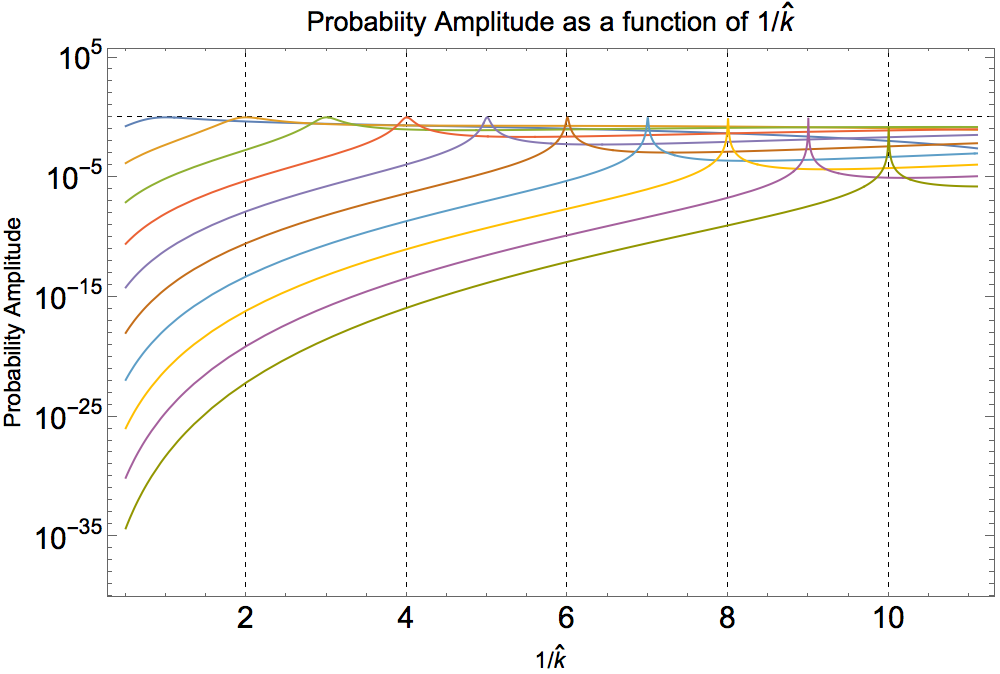
\includegraphics[width=0.95\textwidth]{assets/stimulated-single-frequency-resonances-k-orders.png}
\caption*{Resonances of different $n = 1/\hat k$. Width becomes extremely narrow for high orders.}
\end{figure}

}

\only<2->{
\begin{textblock*}{300pt}(40pt,100pt)
\begin{tcolorbox}
Condition for interference to be important from high orders: width should be larger than a critical value.
\end{tcolorbox}
\end{textblock*}
}





\end{frame}







% \begin{frame}{Single Frequency Matter Profile}

% \begin{figure}
%     \centering
%     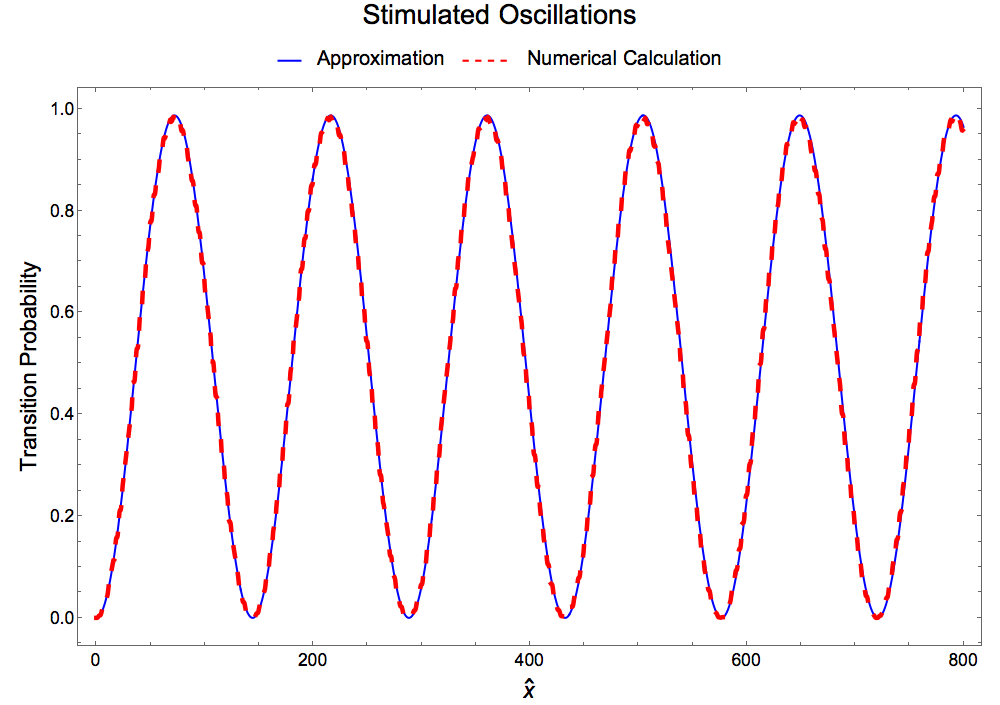
\includegraphics[width=0.9\textwidth]{assets/stimulated-oscillation-rwa-and-numerical.png}
%     \caption*{$\hat A=0.1$, $\hat k=0.995$, $\theta_{\mathrm{m}}=\pi/6$}
% \end{figure}

% \end{frame}



\begin{frame}{Single Frequency Matter Profile Revisited}

Matter profile
\begin{equation*}
    \lambda(x) = \lambda_0 + {\color{red}A \sin (k x)},
\end{equation*}


\only<1>{
\begin{figure}
    \centering
    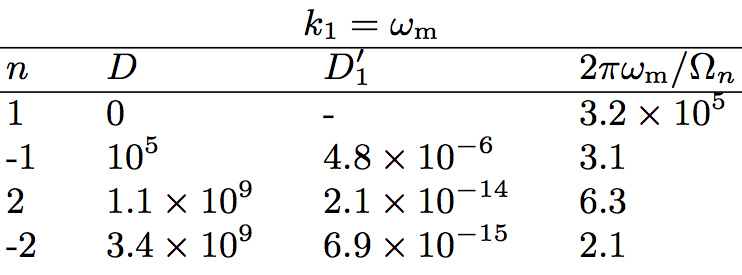
\includegraphics[width=0.9\textwidth]{assets/relative-detuning-and-osc-length-1}
    
\end{figure}
}

\only<2>{
\begin{figure}
    \centering
    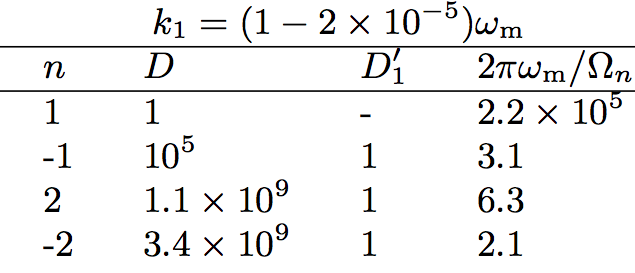
\includegraphics[width=0.9\textwidth]{assets/relative-detuning-and-osc-length-2}
    
\end{figure}
}

\only<3>{
\begin{figure}
    \centering
    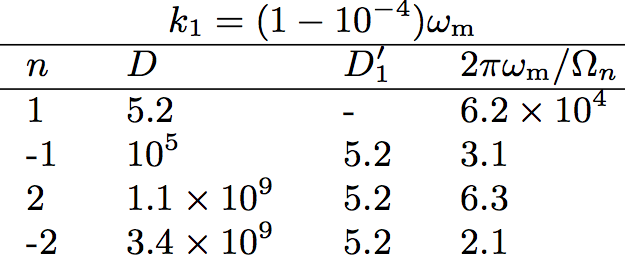
\includegraphics[width=0.9\textwidth]{assets/relative-detuning-and-osc-length-3}
    
\end{figure}
}


\end{frame}




\begin{frame}{Castle Wall Matter Profile}




\begin{columns}[T]
\begin{column}{0.5\textwidth}


\only<1>{
\begin{figure}
    \centering
    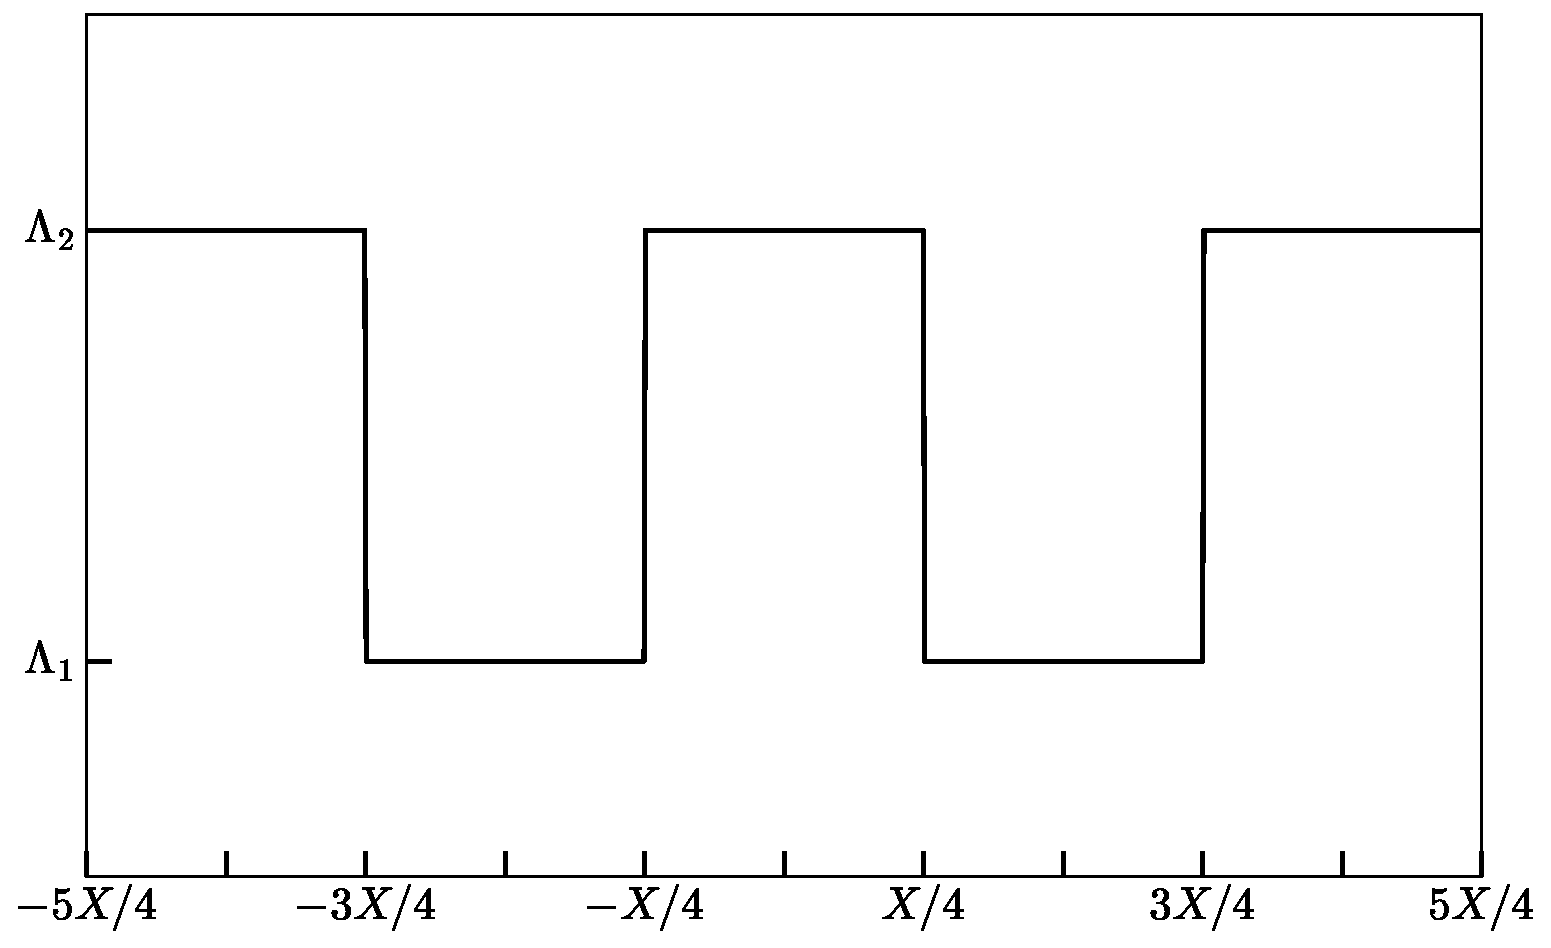
\includegraphics[width=\columnwidth]{assets/castlewall-profile}
    \caption{Castle wall matter profile}
\end{figure}
}


\only<2>{

\begin{table}
\caption{Relative detuning of each frequency.} 
\begin{tabular}{lll} 
 $\{n_1,n_2\}$ &  $D$ & $D'_{\{1,0\}}$   \\
\hline \\
 $\{1,0\}$ & $0$ &  - \\ 
 $\{-1,0\}$ & $48$ &  $1.0\times 10^{-2}$ \\ 
 $\{0,1\}$ & $1.5\times 10^2$ &  $1.1\times 10^{-3}$  \\
 $\{2,0\}$ & $2.4\times 10^{2}$ & $2.0\times 10^{-4}$
\end{tabular} 
\end{table}

}
\end{column}%
\begin{column}{0.5\textwidth}

\begin{figure}
        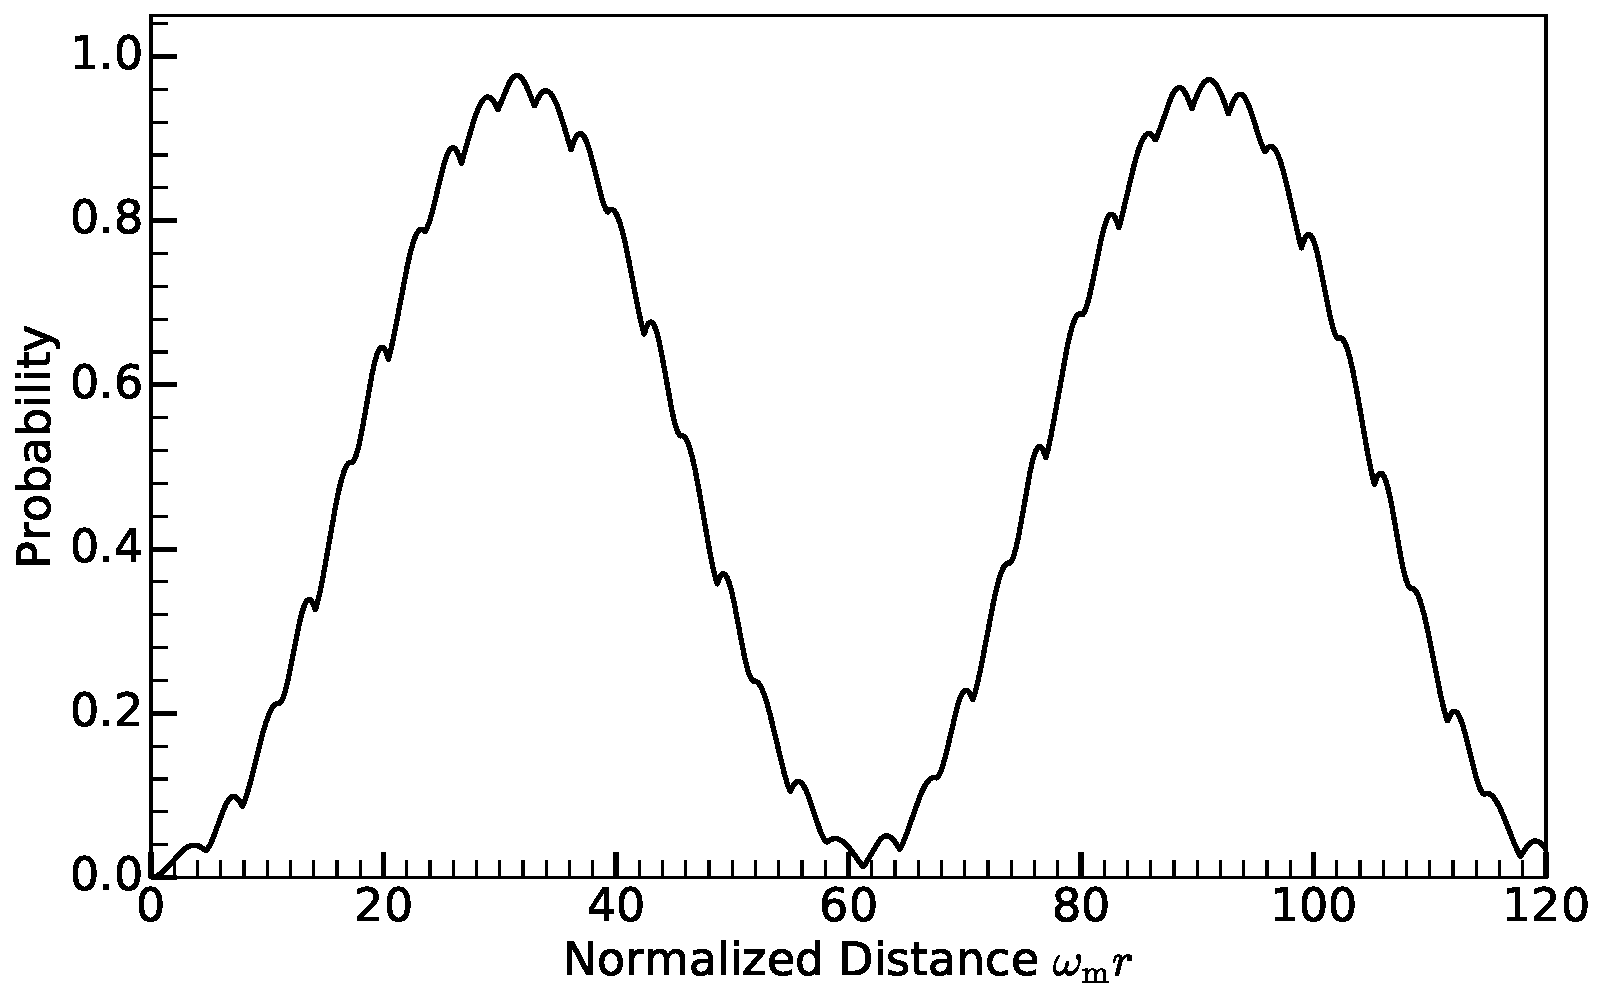
\includegraphics[width=\columnwidth]{assets/castle-wall-1}%
    % \caption{Transition probilities}
\end{figure}


\end{column}
\end{columns}




\end{frame}




%%%%%%%%%%%%%%%%%%%%%%%%%%%%%%%%%%%%%%%%%%%%%%%%%
%%%%%%% Summary & Outlook/Future Work %%%%%%%%%%%%%%

% You should see now what I am trying to do here.
% In reality, a matter profile can be decomposed into many Fourier modes. If we can find a way to determine which terms are important, it would be very useful for more complicated calculations such as the combination of COLLECTIVE neutrino oscillations and matter effect.
% Rather easy to numerically solve such systems. However, it is also good to learn the physics behind numerical calculation. Look into the most important term.

\section{Summary}

\begin{frame}{Summary}


\begin{itemize}\color{ao}
\item 
The fact that neutrino flavor sates are not mass states causes vacuum oscillations.
\item 
MSW resonance happens when matter potential cancels out the vacuum diagonal elements of the Hamiltonian.
\item
Even matter profile doesn't match MSW requirement, variation in matter profile can cause resonances.
\item
Single frequency perturbations in matter profile is a combination of many Rabi oscillations.
\item
Rabi oscillations with two driving fields of different frequencies: large width to destroy the resonance.
\end{itemize}







\end{frame}



% \begin{frame}{Acknowledgement}

% I am very thankful to my advisor Professor Huaiyu Duan, and everyone in our group Dr. Sajad Abbar, and Dr. Shashank Shalgar, for all the help in both research and life.

% Supported by DOE EPSCoR grant \#DE-SC0008142 at UNM.

% \end{frame}







\appendix


\begin{frame}{Backup Slides}

\begin{tcolorbox}
\centering
BACKUP SLIDES
\end{tcolorbox}

\end{frame}



\begin{frame}[fragile]{Why Do Neutrinos Oscillate?}

\begin{tcolorbox}[title=Equation of Motion]

\begin{equation*}
i\partial_x \ket{\Psi} = \hat {\mathbf H} \ket{\Psi}
\end{equation*}

\end{tcolorbox}




\begin{itemize}
\item Basis: Hamiltonian diagonalized basis/mass basis/propagation basis, $\{ \ket{\nu_1}, \ket{\nu_2}\}$.

\item
\begin{equation*}
    \mathbf H = - \frac{\omega_\mathrm v}{2}\boldsymbol{\sigma_3}, \qquad \text{where } \omega_{\mathrm v} = \frac{\delta m^2}{2E}=\frac{m_2^2 - m_1^2}{2E} .
\end{equation*}



\item The system can be solved given initial condition of the amplitudes of the two eigenstates $(\braket{\nu_1}{\Psi(0)},\braket{\nu_2}{\Psi(0)} )^T$,
\begin{equation*}
    \begin{pmatrix}
    \braket{\nu_1}{\Psi(x)} \\
    \braket{\nu_2}{\Psi(x)}
    \end{pmatrix} = \begin{pmatrix}
    \braket{\nu_1}{\Psi(0)} \exp\left( i  \omega_{\mathrm v} x /2 \right) \\
    \braket{\nu_2}{\Psi(0)} \exp\left( -i  \omega_{\mathrm v} x/2 \right)
    \end{pmatrix} 
\end{equation*}


\end{itemize}




\end{frame}


%%%%%%%%%



\begin{frame}[fragile]{Why Do Neutrinos Oscillate?}
\setbeamercovered{invisible}

\begin{tcolorbox}[title=Flavor basis]


Neutrino wave function in flavor basis $\{\ket{\nu_{\mathrm e}}, \ket{\nu_{\mathrm \mu}} \}$ is related to state in energy basis $\{\ket{\nu_1},\ket{\nu_2} \}$ through

\begin{equation*}
\begin{pmatrix}\ket{\nu_{\mathrm e}} \\ \ket{\nu_{\mathrm \mu} } \end{pmatrix} = \begin{pmatrix}  \cos\theta_{\mathrm{v}}  & \sin\theta_{\mathrm{v}} \\ -\sin\theta_{\mathrm{v}}  & \cos\theta_{\mathrm{v}} \end{pmatrix}   \begin{pmatrix}\ket{\nu_1} \\ \ket{\nu_2}\end{pmatrix}
\end{equation*}
$\theta_{\mathrm{v}}$: vacuum mixing angle


\end{tcolorbox}

\pause

\begin{tcolorbox}[title=Hamiltonian $\mathbf H$]

\begin{columns}[T] % align columns
\begin{column}{.49\textwidth}

\centering Mass basis


\begin{align*}
&\frac{\omega_{\mathrm{v}}}{2}\begin{pmatrix}
-1  & 0 \\
0 & 1
\end{pmatrix}\\
=&
-\frac{\omega_{\mathrm v} }{2}\boldsymbol{ \sigma_3 }
\end{align*}



\end{column}%
\hfill%

\begin{column}{.49\textwidth}

\centering Flavor basis

\begin{align*}
&\frac{\omega_{\mathrm v} }{2}\begin{pmatrix} -\cos 2\theta_{\mathrm{v}} & \sin 2 \theta_{\mathrm{v}} \\ \sin 2\theta_{\mathrm{v}} & \cos 2\theta_{\mathrm{v}}  \end{pmatrix} \\
=&
\frac{\omega_{\mathrm v} }{2}\left( - \cos 2\theta_{\mathrm{v}}\boldsymbol{ \sigma_3 } + \sin 2\theta_{\mathrm{v}} \boldsymbol{\sigma_1} \right)
\end{align*}

\end{column}%
\end{columns}

\end{tcolorbox}



\end{frame}





\begin{frame}[fragile]{Nature of Neutrino Oscillation}
\setbeamercovered{invisible}



\begin{tcolorbox}[title=Transition Probability]

\begin{equation*}
P(\ket{\nu_{\mathrm e} }\to\ket{\nu_{\mu}})  =  \sin^2(2\theta_{\mathrm v}) \sin^2 \left( \omega_{\mathrm v} x/2 \right) 
\end{equation*}
\begin{itemize}
    \item $\omega_{\mathrm v}=(m_2^2-m_1^2)/2E$ determines oscillation wavelength.
    \item Mixing angle $\theta_{\mathrm v}$ determines flavor oscillation amplitude.
\end{itemize}




\end{tcolorbox}


\end{frame}





\begin{frame}{MSW Effect}


\begin{textblock*}{10pt}(200pt,1pt)
\small
\begin{equation*}
  \begin{pmatrix}\ket{\nu_{\mathrm e}} \\ \ket{\nu_{\mathrm \mu} } \end{pmatrix} = \begin{pmatrix}  \cos\theta_{\mathrm{v}}  & \sin\theta_{\mathrm{v}} \\ -\sin\theta_{\mathrm{v}}  & \cos\theta_{\mathrm{v}} \end{pmatrix}   \begin{pmatrix}\ket{\nu_1} \\ \ket{\nu_2}\end{pmatrix}
\end{equation*}
\end{textblock*}




Constant matter profile $\lambda_0$ as an example,

\begin{tcolorbox}[title=Significance of $\theta_{\mathrm{m}}$]

Define matter basis (eigenenergy basis) $\{\ket{\nu_{\mathrm{L}}}, \ket{\nu_{\mathrm{H}}}\}$

\begin{equation*}
\begin{pmatrix}
\ket{\nu_{\mathrm{e}}} \\
\ket{\nu_{\mu}}
\end{pmatrix} =
\begin{pmatrix}
\cos\theta_{\mathrm m} & \sin\theta_{\mathrm m} \\
-\sin\theta_{\mathrm m} & \cos\theta_{\mathrm m}
\end{pmatrix}\begin{pmatrix}
\ket{\nu_{\mathrm{L}}} \\
\ket{\nu_{\mathrm{H}}}
\end{pmatrix}
\end{equation*}

\end{tcolorbox}


In matter basis

\begin{equation*}
    \mathbf{H}_{\text{matter-basis}} = -\frac{\omega_{\mathrm m}}{2}\boldsymbol{\sigma_3}
\end{equation*}

\only<2>{

\begin{tcolorbox}[title=Transition Probability]
\begin{equation*}
P(\ket{\nu_{\mathrm{e}}}\to\ket{\nu_\mu})  =  \sin^2(2\theta_{\mathrm{m}}) \sin^2 \left( \omega_{\mathrm{m}} x \right)
\end{equation*}

\end{tcolorbox}


}

\end{frame}








\begin{frame}<presentation:0>[noframenumbering]{MSW Resonance}


\begin{tcolorbox}[title=Hamiltonian with Matter Potential]

\begin{align*}
    \mathbf{H} &= \frac{\lambda(x) -\omega_{\mathrm{v}} \cos 2\theta_{\mathrm{v}} }{2} \boldsymbol{\sigma_3}  + \frac{ \omega_{\mathrm{v}} \sin 2\theta_{\mathrm{v}}}{2}  \boldsymbol{\sigma_1} \\
    &=\frac{ \omega_{\mathrm{m}}(x)    \cos 2\theta_{\mathrm{m}}(x)  }{2} \boldsymbol{\sigma_3} + \frac{ \omega_{\mathrm{m}}(x)    \sin 2\theta_{\mathrm{m}}(x)  }{2} \boldsymbol{\sigma_1}
\end{align*}

\begin{equation*}
\tan 2\theta_{\mathrm{m}}(x) =  \frac{\omega_{\mathrm{v}} \sin 2\theta_{\mathrm{v}}  }{ \omega_{\mathrm{v}}\cos 2\theta_{\mathrm{v}} - \lambda(x)  }.
\end{equation*}


\begin{equation*}
\begin{pmatrix}
\ket{\nu_{\mathrm{e}}} \\
\ket{\nu_{\mu}}
\end{pmatrix} =
\begin{pmatrix}
\cos\theta_{\mathrm m} & \sin\theta_{\mathrm m} \\
-\sin\theta_{\mathrm m} & \cos\theta_{\mathrm m}
\end{pmatrix}\begin{pmatrix}
\ket{\nu_{\mathrm{L}}} \\
\ket{\nu_{\mathrm{H}}}
\end{pmatrix}
\end{equation*}


\end{tcolorbox}





\begin{tcolorbox}[title=Transition Probability]
\begin{equation*}
P(\ket{\nu_{\mathrm{e}}}\to\ket{\nu_\mu})  =  \sin^2(2\theta_{\mathrm{m}}) \sin^2 \left( \omega_{\mathrm{m}} x \right)
\end{equation*}

\end{tcolorbox}





\end{frame}




%%%%%%% MSW Effect %%%%%%%%%

\subsection{Solar Neutrino Problem}

\begin{frame}{Solar Neutrino Problem}

% \begin{tcolorbox}[title=Solar Neutrinos]
% {\color{gray}pp chain}, $\mathrm{{}^7Be}$, $\mathrm{{}^8B}$, pep, CNO
% \end{tcolorbox}

\begin{figure}
    \centering
    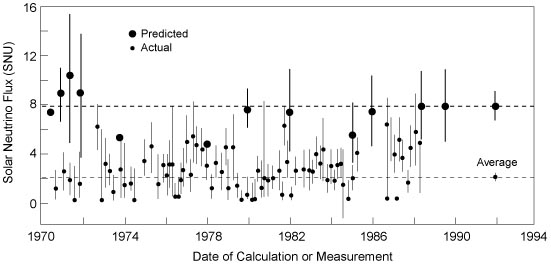
\includegraphics[width=0.9\textwidth]{assets/chlorine-detector-solar-neutrinos.jpg} %https://ase.tufts.edu/cosmos/print_images.asp?id=37
    %https://ase.tufts.edu/cosmos/view_picture.asp?id=585
    \caption*{Chlorine detector (Homestake experiment) results and theory predictions. SNU: 1 event for $10^{36}$ target atoms per second. Kenneth R. Lang (2010)}
\end{figure}


% \begin{figure}
% \centering
% 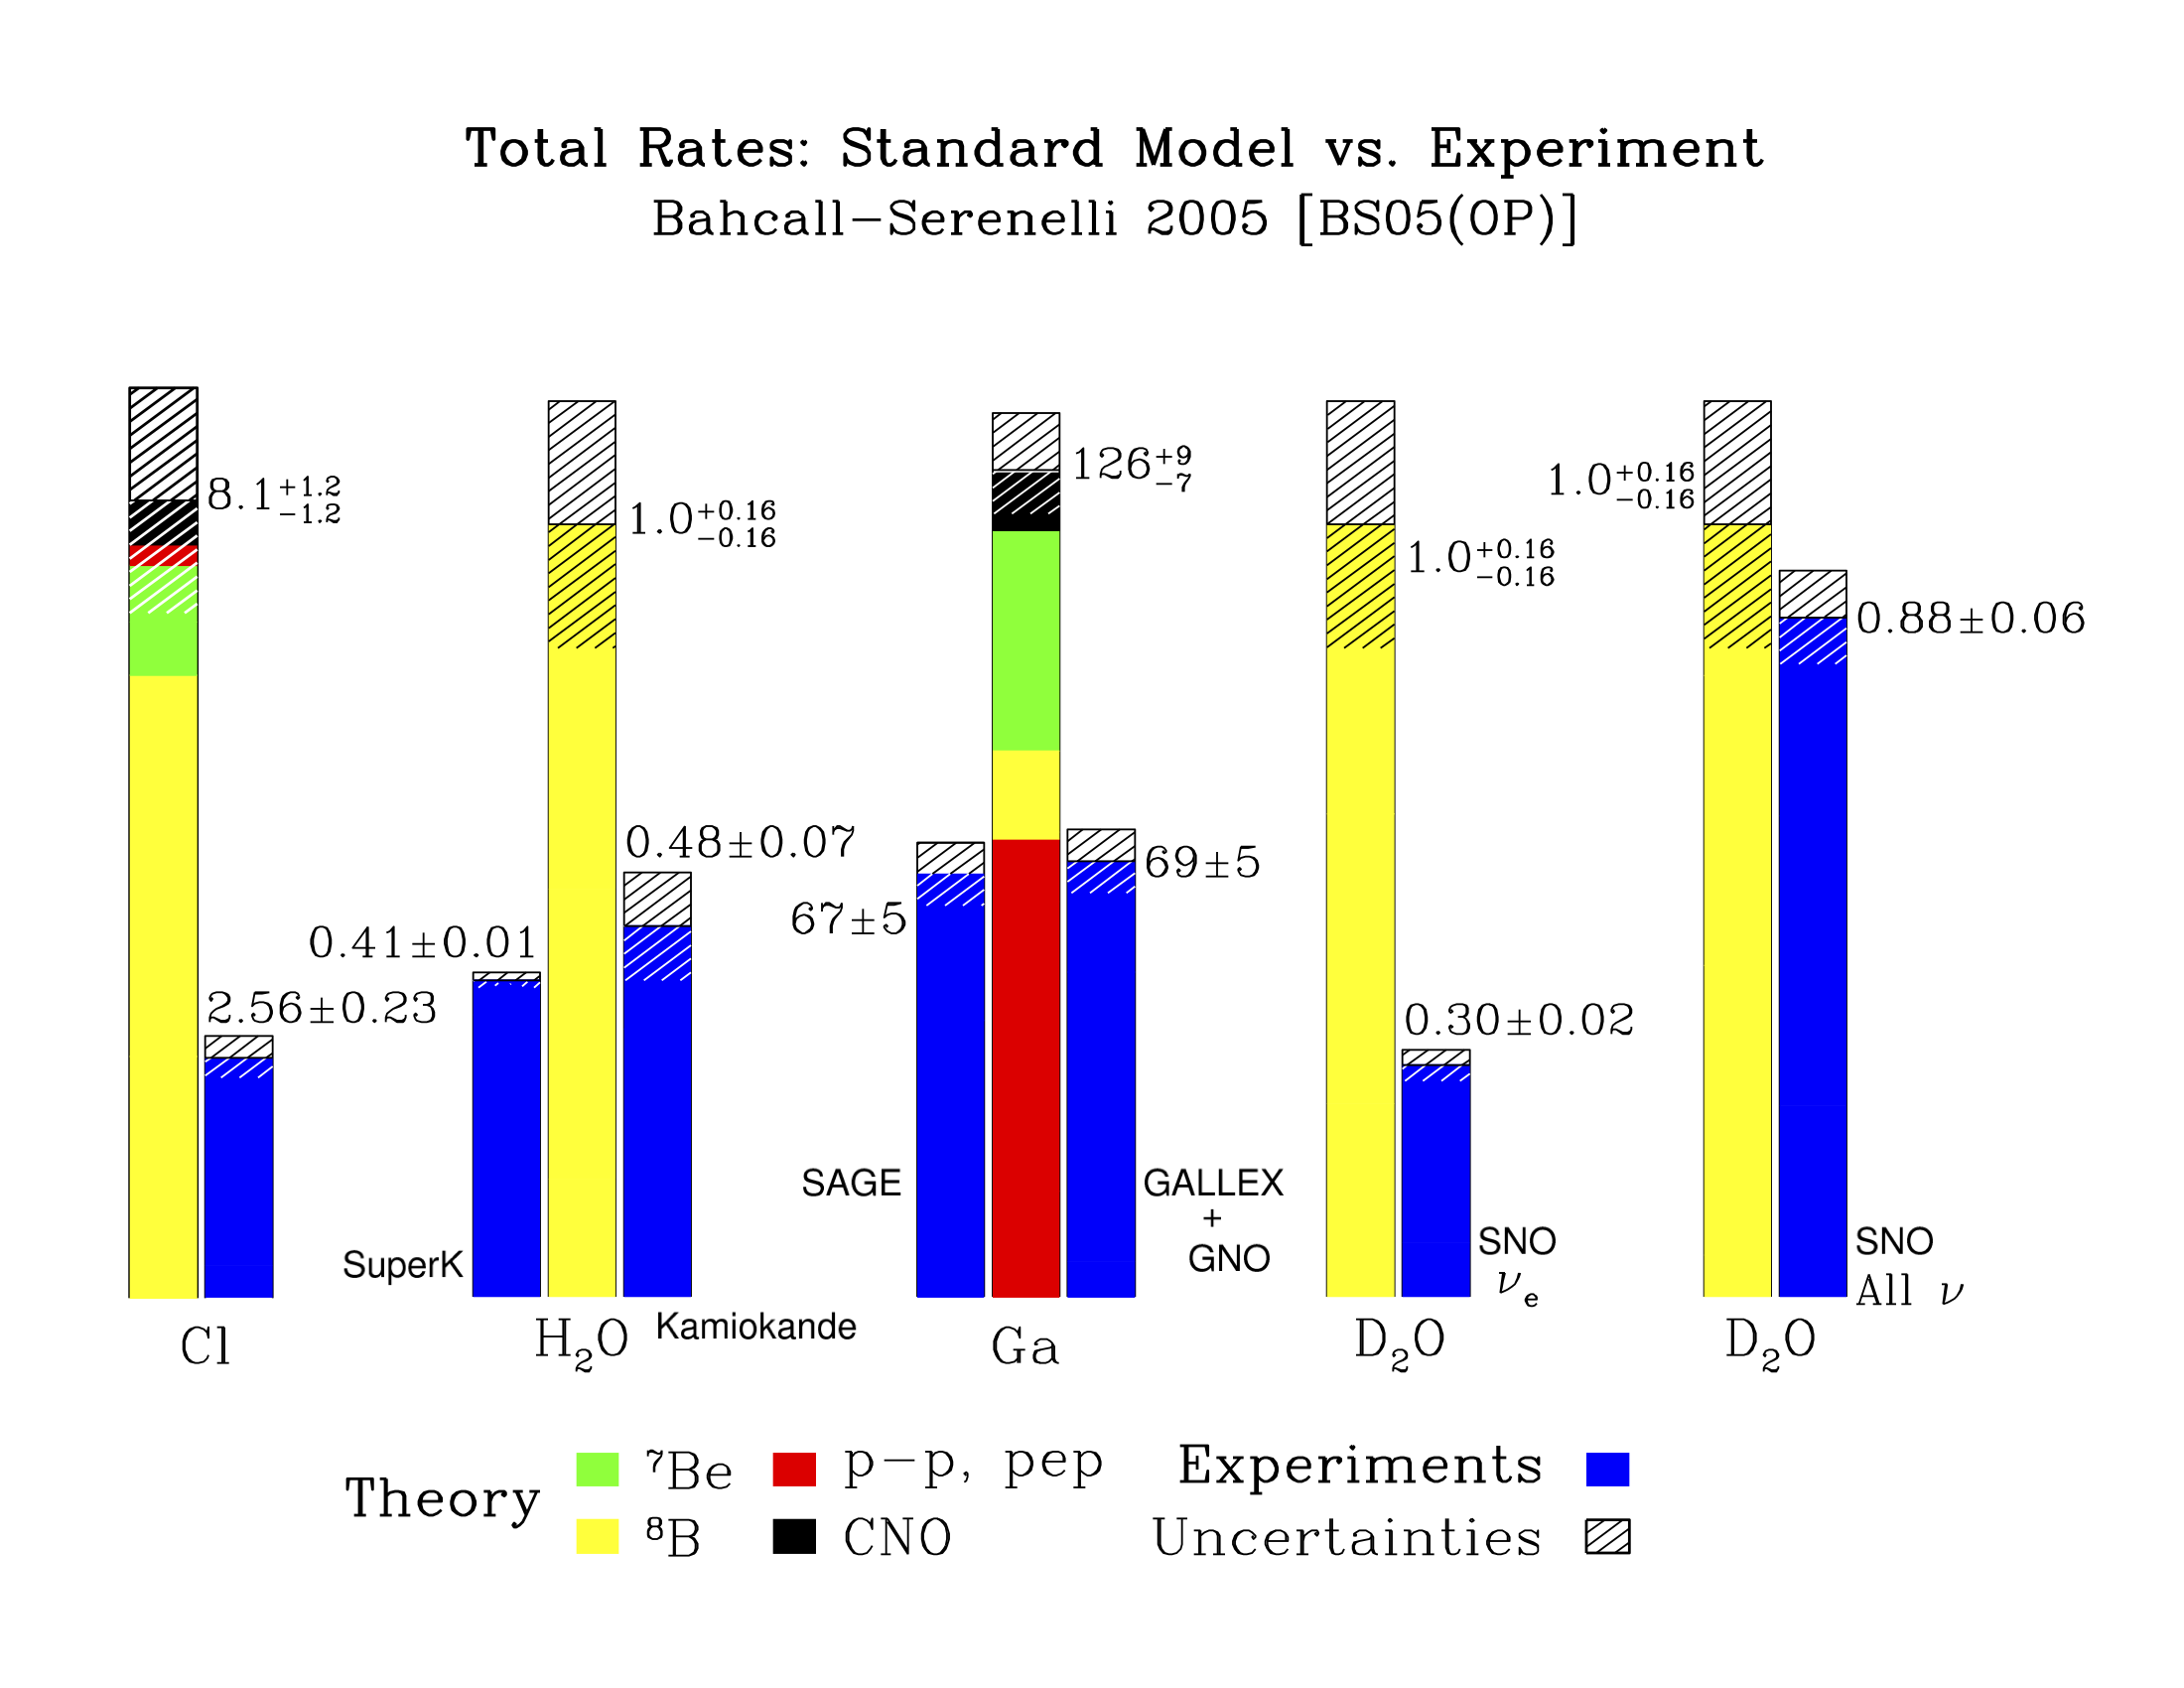
\includegraphics[width=0.8\textwidth]{assets/colortheoryvsexp.png}
% \caption*{Less electron flavor neutrinos observed in experiments than the Standard Solar Model prediction. Bahcall \& Serendelli, 2005}
% \end{figure}


    
\end{frame}

\begin{frame}{MSW Effect and Solar Neutrinos}

\setbeamercovered{invisible}



\begin{equation*}
    \mathbf{H} = \frac{\lambda(x) - \omega_{\mathrm v} \cos 2\theta_{\mathrm v}}{2} \boldsymbol{\sigma_3} + \frac{ \omega_{\mathrm v} \sin 2\theta_{\mathrm v}}{2} \boldsymbol{\sigma_1}
\end{equation*}


\begin{equation*}
\begin{pmatrix}
\ket{\nu_{\mathrm{L}}} \\
\ket{\nu_{\mathrm{H}}}
\end{pmatrix} =
\begin{pmatrix}
\cos\theta_{\mathrm m} & -\sin\theta_{\mathrm m} \\
\sin\theta_{\mathrm m} & \cos\theta_{\mathrm m}
\end{pmatrix}\begin{pmatrix}
\ket{\nu_{\mathrm{e}}} \\
\ket{\nu_{\mu}}
\end{pmatrix}
\end{equation*}




\begin{equation*}
    \mathbf{H}_{\text{matter-basis}} = -\frac{\omega_{\mathrm m}}{2}\boldsymbol{\sigma_3}
\end{equation*}









\begin{figure}
\centering
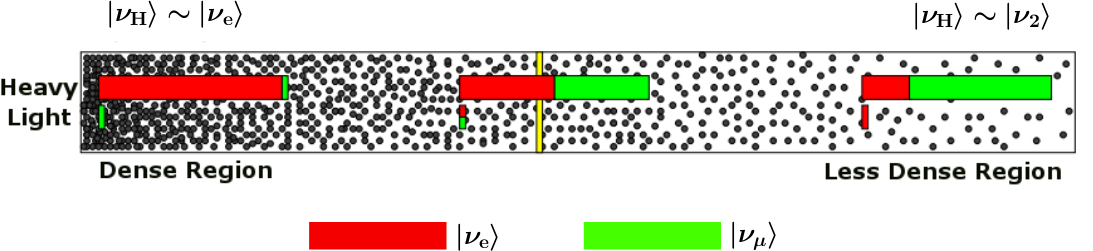
\includegraphics[width=0.9\textwidth]{assets/msw-and-density.png}
\caption*{Yellow bar is the resonance point. Red: $\ket{\nu_e}$. Green: $\ket{\nu_\mu}$. Adapted from Smirnov, 2003.}
\end{figure}



\end{frame}



\begin{frame}{MSW Effect Inverted Hierarchy}


Suppose $\omega_{\mathrm v} = (m_2^2 - m_1^2)/2E <0$,

\begin{equation*}
    \mathbf{H} = \colorbox{blue!20}{$
    -\frac{\omega_{\mathrm{v}}}{2}\begin{pmatrix} -\cos 2\theta_{\mathrm{v}} & \sin 2 \theta_{\mathrm{v}} \\ \sin 2\theta_{\mathrm{v}} & \cos 2\theta_{\mathrm{v}}  \end{pmatrix} 
    $}
             \colorbox{red!20}{$
            + \sqrt{2}G_{\mathrm{F}} n_{\mathrm{e}}(x) \begin{pmatrix}
            1 & 0 \\
            0 & 0
            \end{pmatrix}
            $}
\end{equation*}

\centering
$\big\downarrow$

\begin{equation*}
    \mathbf{H} =
    \left( 
    %\colorbox{blue!20}{$ 
     \frac{-\omega_{\mathrm{v}}}{2} \cos 2\theta_{\mathrm{v}}  
    % $} \colorbox{red!20}{$ 
    + \frac{\lambda(x)}{2}
    % $}
    \right) \boldsymbol{\sigma_3}
    % \colorbox{blue!20}{$ 
            - \frac{\omega_{\mathrm v}}{2}\sin 2\theta_{\mathrm v} \boldsymbol{\sigma_1}
     %       $}
\end{equation*}

\end{frame}


\begin{frame}{Hamiltonian}

\only<1>{
% Matter profile
\begin{tcolorbox}[title=Matter Profile]
\begin{equation*}
    \lambda(x)  = \lambda_0 + {\color{red}\delta\lambda(x)}
\end{equation*}
\end{tcolorbox}


% Basis


\begin{tcolorbox}[title=Basis]

Background matter basis (eigen energy basis): Hamiltonian is diagonalized with only background matter profile $\lambda_0$,

\begin{equation*}
    \mathrm{H}_{\mathrm{background}} = -\frac{\omega_{\mathrm{m}}}{2} \boldsymbol{\sigma_3}.
\end{equation*}

\end{tcolorbox}


% Hamiltonian of with perturbation in matter profile, in background matter basis
\begin{tcolorbox}[title=Hamiltonian]

\begin{equation*}
    \mathbf H = \frac{1}{2}\left( - \omega_{\mathrm{m}} + {\color{red}\delta \lambda(x)} \cos 2\theta_{\mathrm{m}} \right) \boldsymbol{\sigma_3} - \frac{{\color{red}\delta \lambda(x) } }{2} \sin \theta_{\mathrm{m}} \boldsymbol{\sigma_1}.
\end{equation*}


\end{tcolorbox}

}

\only<2>{

\begin{tcolorbox}[title=Hamiltonian in Background Matter Basis]
    \begin{equation*}
    \mathbf {H} = \frac{1}{2}\left( - \omega_{\mathrm{m}} + {\color{red}\delta \lambda(x)} \cos 2\theta_{\mathrm{m}} \right) \sigma_3 - \frac{  {\color{red}\delta \lambda(x)}  }{2} \sin 2\theta_{\mathrm{m}} \sigma_1.
\end{equation*}
\end{tcolorbox}


Matter profile
\begin{equation*}
    \lambda(x) = \lambda_0 + {\color{red}A \cos (k x)},
\end{equation*}


\begin{equation*}
    \mathbf {H} = \frac{1}{2}\left( - \omega_{\mathrm{m}} +  \cos 2\theta_{\mathrm{m}}{\color{red}A\cos(kx)} \right) \sigma_3 - \frac{  \sin 2\theta_{\mathrm{m} }  }{2}{\color{red}A \cos(kx)}  \sigma_1.
\end{equation*}

}

\only<3>{

\begin{tcolorbox}[title=Hamiltonian in Background Matter Basis]
    \begin{equation*}
    \mathbf {H} = \frac{1}{2}\left( - \omega_{\mathrm{m}} + {\color{red}\delta \lambda(x)} \cos 2\theta_{\mathrm{m}} \right) \sigma_3 - \frac{  {\color{red}\delta \lambda(x)}  }{2} \sin 2\theta_{\mathrm{m}} \sigma_1.
\end{equation*}
\end{tcolorbox}


Matter profile
\begin{equation*}
    \lambda(x) = \lambda_0 + {\color{red}A \cos (k x)},
\end{equation*}


\begin{equation*}
    \mathbf {H} = \frac{1}{2}\left( - \omega_{\mathrm{m}} \colorbox{gray!20}{$+  \cos 2\theta_{\mathrm{m}}{\color{red}A\cos(kx)} $} \right) \sigma_3 - \frac{  \sin 2\theta_{\mathrm{m} }  }{2}{\color{red}A \cos(kx)}  \sigma_1.
\end{equation*}

}




\end{frame}


\begin{frame}{Rabi Oscillations}


The coupling strength is calculated as

\begin{equation*}
    \alpha = \langle 1 \vert \mathbf d \cdot \mathbf E \vert 2 \rangle
\end{equation*}

where the electric field is 

\begin{equation*}
    \mathbf E = \mathbf E_0 \sin(k t).
\end{equation*}

and $\mathbf d$ is the dipole moment.

\end{frame}

\begin{frame}{Visualizing Rabi Oscillations}

\begin{textblock*}{10pt}(250pt,1pt)
\small
\begin{equation*}
  % The Pauli matrices form
  %-\frac{\omega_0}{2} \sigma_3 - \frac{\alpha}{2} \cos(kt)\sigma_1 + \frac{\alpha}{2}\sin(kt)\sigma_2
  % The single matrix form
   -\frac{\omega_0}{2} \sigma_3 - \frac{\alpha}{2} \begin{pmatrix}
    0 & e^{ikt}\\
    e^{-ikt} & 0
    \end{pmatrix}
\end{equation*}
\end{textblock*}



\begin{columns}[T]
\begin{column}{0.6\textwidth}

\begin{align*}
    &-\frac{\omega_0}{2} \sigma_3 - \frac{\alpha}{2} \cos(kt) \sigma_1 + \frac{\alpha}{2}\sin(kt) \sigma_2 \\
= & \begin{pmatrix}
\alpha \cos(kt) &
-\alpha \sin(kt) &
\omega_0
\end{pmatrix}
\colorbox{blue!20}{$\begin{pmatrix}
-\sigma_1/2 \\
-\sigma_2/2 \\
-\sigma_3/2
\end{pmatrix}
$} \\
=& \vec H \cdot (-\vec{\sigma}/2)
\end{align*}

\end{column}%
\begin{column}{0.4\textwidth}
\begin{figure}
    \centering
    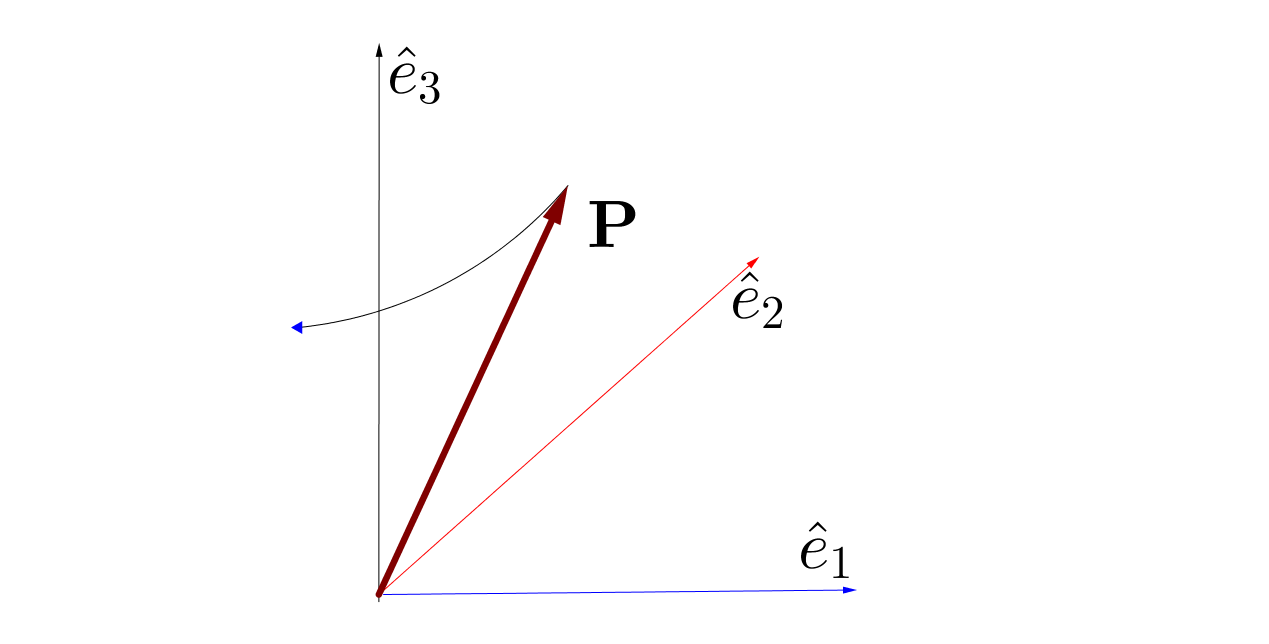
\includegraphics[width=\textwidth,trim={2cm 0 3cm 0},clip]{assets/rabi-bloch-vector-rotation}
\end{figure}


\end{column}
\end{columns}


\begin{equation*}
    D = \left\vert\frac{\omega_0 - k}{\alpha} \right\vert
\end{equation*}

is ratio of the energy gap in corotating frame to width of resonance.

\end{frame}


\begin{frame}{Interferences of Rabi Oscillations}

\begin{textblock*}{10pt}(250pt,1pt)
\small
\begin{equation*}
  % The Pauli matrices form
  %-\frac{\omega_0}{2} \sigma_3 - \frac{\alpha}{2} \cos(kt)\sigma_1 + \frac{\alpha}{2}\sin(kt)\sigma_2
  % The single matrix form
   -\frac{\omega_0}{2} \sigma_3 - \frac{\alpha}{2} \begin{pmatrix}
    0 & e^{ikt}\\
    e^{-ikt} & 0
    \end{pmatrix}
\end{equation*}
\end{textblock*}


\begin{align*}
    \mathbf {H} =& \frac{1}{2}\left( - \omega_{\mathrm{m}} \colorbox{gray!20}{$+  \cos 2\theta_{\mathrm{m}}A\cos(kx) $} \right) \sigma_3 - \frac{  \sin 2\theta_{\mathrm{m} }  }{2}A \cos(kx)  \sigma_1\\
    \to& -\frac{\omega_m}{2} \sigma_3 - \frac{A\sin 2\theta_{\mathrm m}}{2} \cos(kx)\sigma_1 \\
    =&-\frac{\omega_m}{2} \sigma_3 - \frac{A\sin 2\theta_{\mathrm m}}{2} \frac{1}{2}\begin{pmatrix}
    0 & e^{ikx}\\
    e^{-ikx} & 0
    \end{pmatrix}
    - \frac{A\sin 2\theta_{\mathrm m}}{2} \frac{1}{2}\begin{pmatrix}
    0 & e^{i(-k)x} \\
    e^{-i(-k)x} & 0
    \end{pmatrix}
\end{align*}

\end{frame}


\begin{frame}{Parameters Used for Vacuum Oscillations}

$\theta_{12} = 33.36/180\pi$;
$\theta_{13} = 8.66/180\pi$;
$\theta_{23} = 40/180*\pi$;
$\delta_{cp} = 0$;
$m_1^2 = 0.01$;
$m_2^2 = m_1^2 + 0.000079$;
$E=1$MeV


\end{frame}



\begin{frame}{Single Frequency Matter Profile}


\only<1-1>{

\begin{tcolorbox}[title=Why Does It Work?]

\begin{equation*}
    J_n(n \sech \alpha) \sim \frac{ e^{ - n(\alpha -\tanh\alpha )} }{ \sqrt{ 2\pi n \tanh \alpha } }, \quad \text{for large } n
\end{equation*}

% Hamiltonian off-diagonal element amplitude

% \begin{equation*}
%     \hat B_n \propto n J_n(n \sech \alpha) \sim \sqrt{n} \frac{ e^{ - n(\alpha -\tanh\alpha )} }{ \sqrt{ 2\pi  \tanh \alpha } }, \quad \text{for large } n
% \end{equation*}

% where $\sech\alpha = \hat A\cos 2\theta_{\mathrm{m}}$.

$\Rightarrow$

\begin{equation*}
    \Gamma \propto \hat B_n \propto  \frac{ e^{ - n ( \alpha - \tanh \alpha )} }{\sqrt{2\pi n \tanh \alpha} } 
\end{equation*}

Small perturbation $\Rightarrow$ Small $\hat A$ $\Rightarrow$ Large $\alpha$ $\Rightarrow$ Drops fast at large $n$.


\end{tcolorbox}
}

\end{frame}







\begin{frame}{Two-frequency Matter Profile}


\only<1-1>{
\begin{tcolorbox}[title=Matter Profile]

\begin{equation*}
    \lambda(x) = \lambda_0 + \color{red}\delta\lambda(x),\quad     \color{red}\delta \lambda(x) = A_1 \sin (k_1 x) +  A_2 \sin (k_2 x).
\end{equation*}
\end{tcolorbox}
}

\only<2->{
\begin{tcolorbox}[title=Hamiltonian Off-diagonal Element]

Apply Jacobi-Anger expansion,

\begin{equation*}
\hat h  = \sum_{n_1=-\infty}^\infty \sum_{n_2=-\infty}^{\infty}  \frac{1}{2} \hat B_{n_1,n_2}(\hat k_1,\hat k_2)
 e^{i(n_1 \hat k_1 + n_2 \hat k_2 - 1)\hat x},
\end{equation*}

where

\begin{align*}
&\hat B_{n_1,n_2}( \hat k_1,\hat k_2)\\
= & -(-i)^{n_1+n_2} ( n_1 \hat k_1 + n_2 \hat k_2 ) J_{n_1}\left( \frac{\hat A_1\cos 2\theta_{\mathrm{m}}}{\hat k_1} \right) J_{n_2}\left( \frac{\hat A_2\cos 2\theta_{\mathrm{m}}}{\hat k_2} \right) 
\end{align*}


\end{tcolorbox}
}


\only<2->{
\begin{tcolorbox}
\centering
\color{red}Which terms are important?
\end{tcolorbox}

}

\only<2->{

\begin{textblock*}{64mm}(68mm,0.01\textheight)

\small
\begin{equation*}
\hat h=\sum_{n=-\infty}^{\infty} \frac{1}{2} \hat B_n e^{i  {\color{magenta} (n\hat k-1) } \hat x},
\end{equation*}
\normalsize

\end{textblock*}


}




\end{frame}


\begin{frame}{Two-frequency Matter Profile}

\only<1-1>{
\begin{tcolorbox}[title=Resonance Lines]

There are still resonances, i.e., (almost) zero phases, on lines

\begin{equation*}
    n_{1,0} \hat k_1 + n_{2,0} \hat k_2 -1 =0
\end{equation*}

in $\{\hat k_1,\hat k_2\}$ plane. 
{\centering
$\Rightarrow$
}
Resonance width for each point on resonance lines.

\end{tcolorbox}
}

\only<2-2>{

\begin{figure}
    \centering
    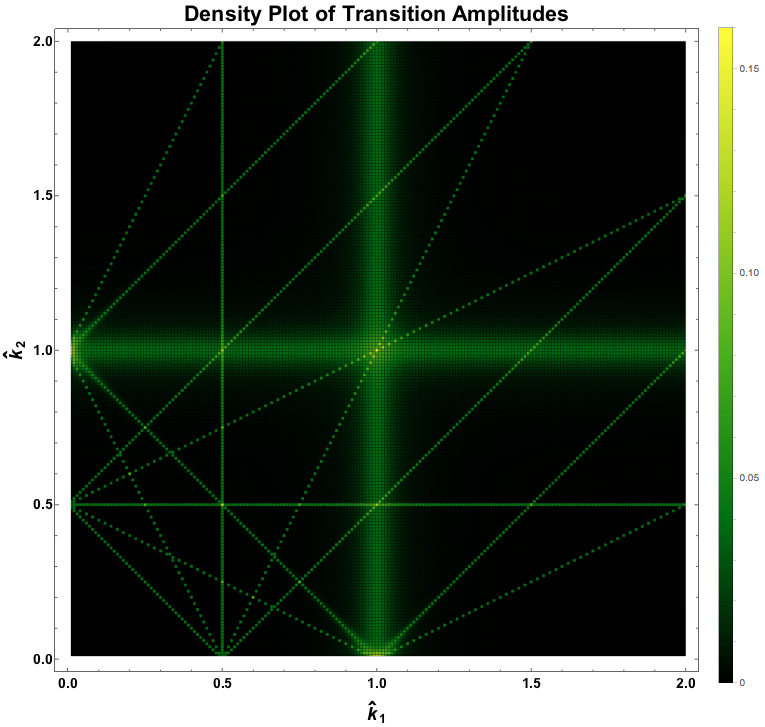
\includegraphics[width=0.7\textwidth]{assets/density-plot-of-transition-amplitudes-demonstration.png}
    \caption*{Density plot of transition amplitudes calculated using only one term out of the whole summation in Hamiltonian. $n_1,n_2\in [-2, 2]$}
\end{figure}

\begin{textblock*}{64mm}(70mm,0.01\textheight)
\tiny
\begin{equation*}
\hat h  = \sum_{n_1} \sum_{n_2}  \frac{1}{2} \hat B_{n_1,n_2}(\hat k_1, \hat k_2)
 e^{i(n_1 \hat k_1 + n_2 \hat k_2 - 1)\hat x},
\end{equation*}
\normalsize
\end{textblock*}

}


\only<3->{
\begin{figure}
    \centering
    \includegraphics[width=0.75\textwidth]{assets/stimulated-2-freq-width-diagram.png}
    \caption*{Resonance line, distance to resonance, and width}
\end{figure}
}



\end{frame}



\begin{frame}{Two-frequency Matter Profile}


\begin{tcolorbox}[title=Width]

\begin{equation*}
    \Gamma_2 = \frac{\hat B_{n_1,n_2}(\hat k_{1,\mathrm{intercept}}, \hat k_{2,\mathrm{intercept}})}{\sqrt{n_1^2 + n_2^2}}.
\end{equation*}

\end{tcolorbox}


\begin{tcolorbox}[title=Distance to Resonance Line]

\begin{equation*}
d = \frac{\lvert n_1 \hat k_{10} + n_2 \hat k_{20} - 1 \rvert}{\sqrt{n_1^2 + n_2^2} }.
\end{equation*}

\end{tcolorbox}


\begin{tcolorbox}[title=Distance to Resonance Width Ratio]

\begin{equation*}
Q_2 = \frac{d}{\Gamma_2}.    
\end{equation*}


\end{tcolorbox}

\end{frame}


\begin{frame}{Two-frequency Matter Profile}



\only<1-1>{
\begin{figure}
    \centering
    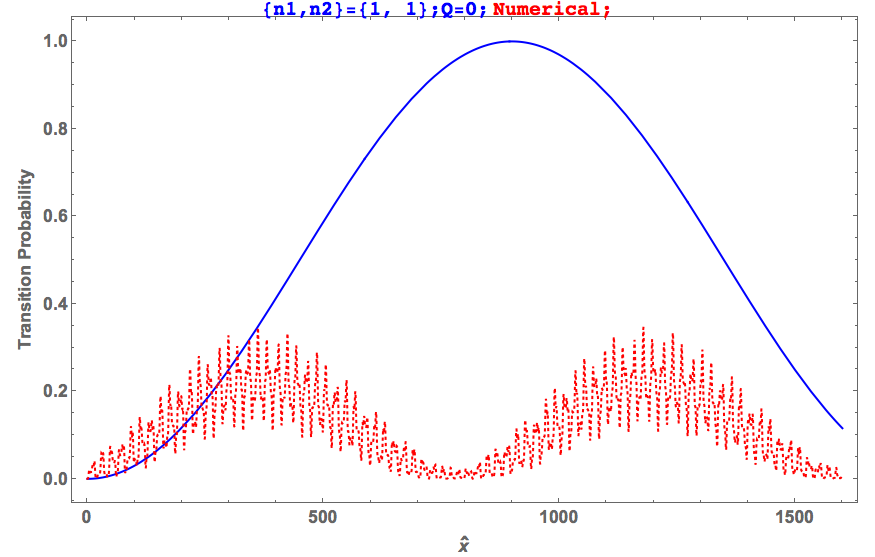
\includegraphics[width=0.9\textwidth]{assets/q-ordering-1.png}
    \caption*{}
\end{figure}
}


\only<2-2>{
\begin{figure}
    \centering
    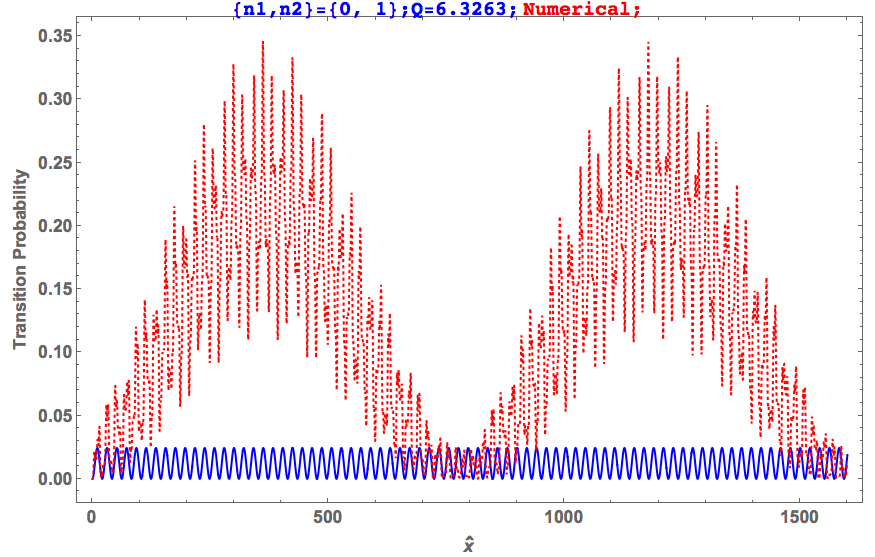
\includegraphics[width=0.9\textwidth]{assets/q-ordering-2.png}
    \caption*{}
\end{figure}
}


\only<3-3>{
\begin{figure}
    \centering
    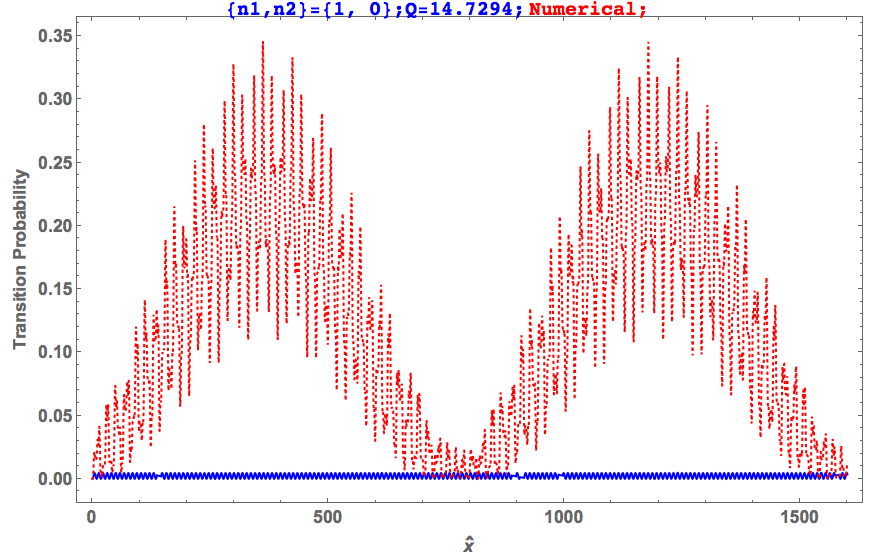
\includegraphics[width=0.9\textwidth]{assets/q-ordering-3.png}
    \caption*{}
\end{figure}
}

\only<4-4>{
\begin{figure}
    \centering
    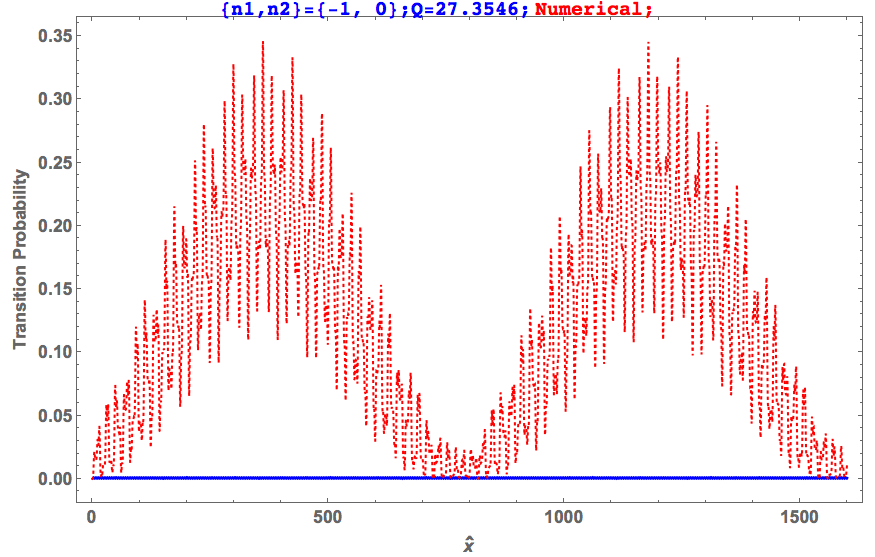
\includegraphics[width=0.9\textwidth]{assets/q-ordering-4.png}
    \caption*{}
\end{figure}
}

\only<5-5>{
\begin{figure}
    \centering
    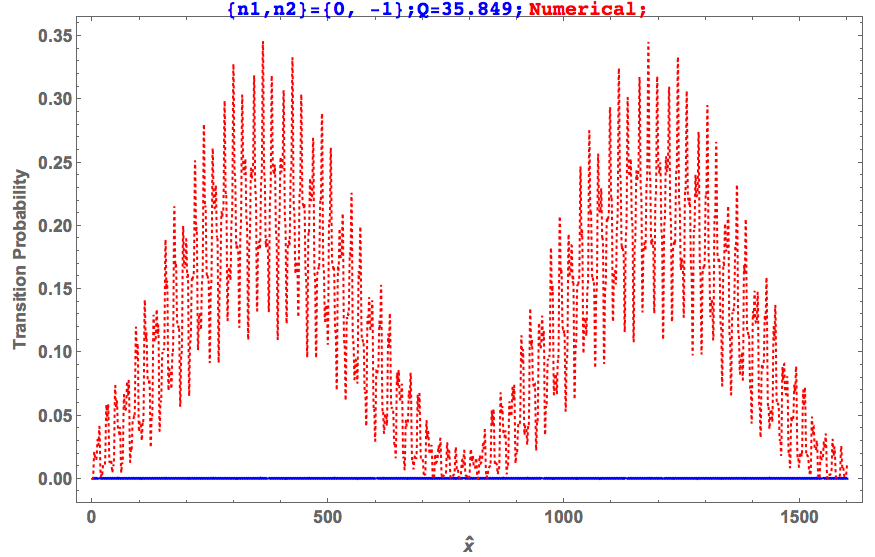
\includegraphics[width=0.9\textwidth]{assets/q-ordering-5.png}
    \caption*{}
\end{figure}
}

\only<6-6>{
\begin{figure}
    \centering
    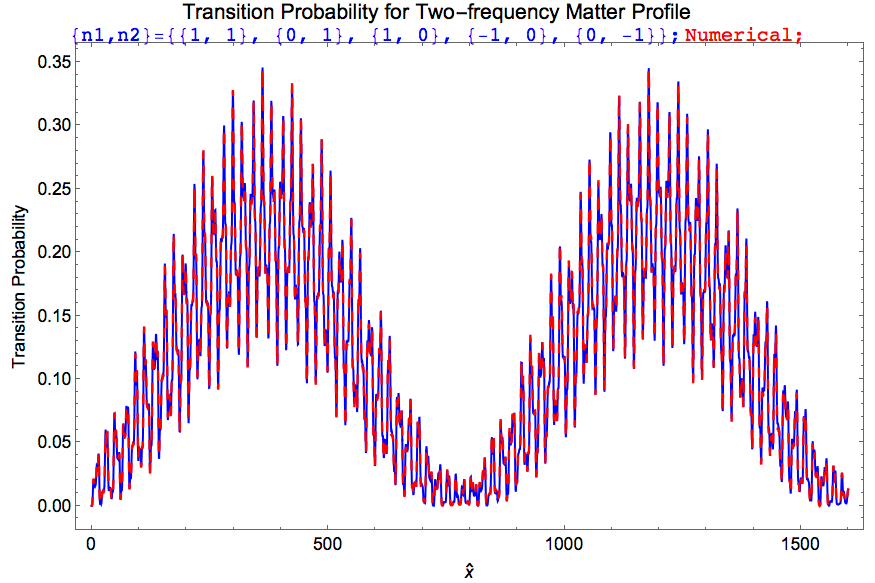
\includegraphics[width=0.9\textwidth]{assets/2-freq-numerical-and-first-5-rwa.png}
    \caption*{}
\end{figure}
}

\end{frame}



\begin{frame}{Bessel's Function}


\begin{equation*}
    J_n(\beta) = \sum_{m=0}^\infty \frac{(-1)^m}{m! \, \Gamma(m+n+1)} {\left(\frac{\beta}{2}\right)}^{2m+n} 
\end{equation*}


\end{frame}



\begin{frame}[allowframebreaks]{References}

  \bibliography{ref}
  \bibliographystyle{abbrv}

\end{frame}

\end{document}
